\documentclass[11pt,a4paper]{article}

% Packages
\usepackage{fontspec}
\setmainfont{Hiragino Mincho ProN}
\setsansfont{Hiragino Kaku Gothic ProN}
\setmonofont{Menlo}
\usepackage{iftex}
\ifXeTeX
  \XeTeXlinebreaklocale "ja"
  \XeTeXlinebreakskip=0pt plus 1pt minus 0.1pt
\fi
\usepackage{amsmath,amssymb,amsthm}
\usepackage{graphicx}
\usepackage{hyperref}
\usepackage{booktabs}

\newtheorem{theorem}{定理}
\newtheorem{definition}{定義}

\title{情報損失としての構造崩壊：\\累積制約下の指数減衰メカニズム}
\author{Akihito Sunagawa\thanks{akihito.sunagawa@gmail.com}}
\date{2026年3月}

\begin{document}

\maketitle

\begin{abstract}
大規模言語モデル（LLM）は、構造的矛盾がコンテキストに蓄積すると推論が突然崩壊する---事実的ノイズ下での緩やかな劣化とは質的に異なる現象である。制御された実験（5ベンダーの11モデル、4B--70B以上のパラメータ）を通じてこの崩壊を特徴づけ、以下を発見した：(i) コンテキストマージン（$\mu$）と構造的矛盾（$\delta$）の間の乗法的交互作用---個別には致死的でない2つのストレッサーが組み合わさると致死的になり、加法的劣化モデルを排除する；(ii) $\delta$における次元構造---十分なベースライン精度を持つモデルにおいて、単一の構造的矛盾が10個の事実的矛盾よりも大きな損害を与える；(iii) クッション機構---RLHFアラインメントが矛盾を圧倒されるまで吸収し、システム固有の臨界閾値$\delta_c$を生じる。

これらのパターンは組合せ論の第一モーメント法により説明される。累積情報損失$\delta = \sum_i I(\text{constraint}_i)$をナット単位で定義すると、乗法的存続ポテンシャル
\[
S = N_{eff} \cdot \frac{\mu}{\mu_c} \cdot e^{-\delta}
\]
はLLMの崩壊パターンを捉えるとともに、$\delta$が正確に計算可能なブール充足可能性（SAT）においてパラメータフリー予測を与える：減衰率比$\alpha_{\text{XOR}}/\alpha_{\text{random}} = \ln 2 / |\ln(7/8)| = 5.19\times$は上界であり、実験的に確認された（観測値：$5.04 \pm 0.25$、CV $= 5\%$；系統的な下方偏差は制約間相関が有効情報損失を減少させることと整合する---制約の重複が冗長性を生み、一箇所の違反がシステム全体に与える影響を緩和する）。指数ペナルティ$e^{-\delta}$は近似ではなく、SAT解の個数の第一モーメントとの数学的恒等式である。その貢献は操作的方法論---構造的矛盾を第一モーメント対応を通じてナット単位の情報損失として測定すること---であり、2つの制御されたドメインで検証された。系統的な$\delta = 0$対照実験（4ベンダー6モデル、500〜128{,}000トークン）は補完的予測を確認する：構造矛盾ゼロの下では十分なベースライン能力（$\mu$）を持つモデルがコンテキスト長に関わらず完璧な正答率を維持する一方、低$\mu$モデル（Llama~3.1:8b）は36\%に留まり、乗法構造$S = \mu \cdot e^{-\delta}$を確認した。追加実験では256{,}000トークンまで3水準の$\delta$（ゼロ、ソース間の微小な食い違い、構造的自己矛盾）を2ベンダー3モデルで交差させた（$n = 810$試行）。これにより\emph{能力--脆弱性パラドックス}が明らかになった：最低能力モデル（GPT-4.1~Nano）は微小矛盾（$\delta_5$）を完全に無視し（\texttt{wrong\_val\_adopted} $= 0/90$）、高能力モデル（GPT-4.1~Mini）は壊滅的に脆弱であり（$\delta_5$下で$37\% \to 7\%$、\texttt{wrong\_val\_adopted} $= 29/90$）、クロスベンダーモデル（Gemini~3.1~Flash-Lite~Preview）は第三のパターンを示す：$\delta_5$感受性がコンテキスト長とともに\emph{減少}（$57\% \to 90\%$、\texttt{wrong\_val\_adopted}は33\%→7\%）し、情報希釈と整合する。構造矛盾（$\delta_1$）は両OpenAIモデルで完全崩壊（$0\%$）を引き起こす一方、Geminiは32Kで$40\%$を達成するが自己参照矛盾を文字通りの再代入として解釈する---質的に異なる失敗モードである。第二モーメント法（Paley--Zygmund不等式）への拡張により、ペア相関関数$g(\beta) = 3/4 + (1/8)(1-\beta)^3$を用いて、第一モーメント上界（$\alpha \approx 5.19$）と真の3-SAT閾値（$\alpha \approx 4.27$）のギャップの74\%を定量的に説明した。残り26\%はレプリカ対称性の破れに帰属される。多重アトラクター拡張---各アトラクター盆地が独自の存続ポテンシャルを持ち$-\ln S$が自由エネルギーの役割を果たす---は遷移点公式$m^* = \ln(C_A/C_B)/(I_A - I_B)$を導出し、Geminiの矛盾感受性が$P(\text{correct}) = 1/(1 + K/L)$（$K \approx 20$千トークン、$L$はコンテキスト長）に従うことを予測する。この予測は確認実験前に3データ点から導出され、5つのコンテキスト長（32K--512K）で平均絶対誤差2\%で一致した。これは多重アトラクター枠組みの最初の定量的検証である。第二モーメントのoverlap分解と多重アトラクター遷移定理を含む全結果はLean~4で機械検証済み（20モジュール、\texttt{sorry}なし、公理なし）。

\medskip
\noindent\textbf{キーワード：} LLM推論崩壊、構造的矛盾、情報損失、乗法モデル、SAT相転移、生存分析、形式検証
\end{abstract}

%=============================================
\section{はじめに}

情報を処理するシステムは、内部矛盾が蓄積すると突然失敗しうる。大規模言語モデルにおいて、これは突然の推論崩壊として現れる：十分なベースライン精度を持つモデルにおいて、単一の構造的矛盾---自己言及パラドックス、メタレベルの不整合---が10個の事実的矛盾よりも大きな損害を与える（第\ref{sec:llm-delta-structure}節）。個別には無害な2つのストレッサー（適度なコンテキスト負荷と適度な矛盾）が組み合わさると致死的になる（第\ref{sec:llm}節）。4Bから70B以上のパラメータを持つ5ベンダーの11モデルにわたり再現された（第\ref{sec:cross-model}節）これらのパターンは、注意機構の劣化や誤差伝播のような加法的劣化モデルでは説明できない---それらは各ストレッサーに独立に比例するパフォーマンス低下を予測する。この現象は、再帰的訓練データ下でのモデル崩壊\cite{shumailov2024}（分布の狭窄として現れる累積情報損失）とは関連しつつも区別される。

なぜ加法的ではなく乗法的なのか？ 本稿はその答えが組合せ論の第一モーメント法という既知の数学的構造にあると提案する。\textbf{累積情報損失}$\delta = \sum_i I(\text{constraint}_i)$をナット単位で定義し、各構造的制約が計算可能な量の情報損失を寄与する。存続ポテンシャルは次の通りである：
\begin{equation}
S = N_{eff} \cdot \frac{\mu}{\mu_c} \cdot e^{-\delta}
\label{eq:survival}
\end{equation}
ここで$N_{eff}$は有効選択肢数（システムが利用可能な独立した代替選択肢の数）、$\mu/\mu_c$は臨界閾値に対するマージン、$e^{-\delta}$は蓄積された構造的矛盾からの指数ペナルティである。いずれかの因子がゼロに近づけば他に関係なく致命的になるこの乗法構造は、直列信頼性\cite{barlow1975}、原子炉臨界\cite{duderstadt1976}、および感染症閾値（$R_0$）の構造である。注目すべきことに、同様の分離は信用評価において独立に制度化されている：主要格付機関（S\&P、Moody's、Fitch）は定量的財務健全性（$\mu$）と定性的ガバナンス要因（$\delta$）を区別しており、Moody'sは「支払能力」と「支払意思」を明示的に分離する---理論的動機なしに数十年の実務を通じて到達したキャパシティ--制約分解である\cite{cantor1996}。

本稿の貢献は乗法構造そのものではなく、情報理論的基盤付けにある：$\delta$を第一モーメント法を通じてナット単位で操作的に定義することで、制約の量だけでなく質が第一原理から計算可能になる。ブール充足可能性（SAT）において、$e^{-\delta}$は解の個数の第一モーメントと数学的に同一である（第\ref{sec:first-moment}節）。この恒等式はパラメータフリー予測を与える：XOR制約はランダム節の$\ln 2 / \ln(8/7) \approx 5.19$倍低い密度で崩壊を引き起こすはずであり---$5.04 \pm 0.25$で実験的に確認された（CV $= 5\%$；第\ref{sec:sat}節）。同じ数学的構造が、LLMにおいて構造的矛盾が事実的ノイズよりも質的に大きな損害を与える理由を説明する：制約あたりの情報損失がより大きいのである。

\subsection{研究課題}

\begin{enumerate}
    \item \textbf{操作的定義}：構造的矛盾を、確立された数学との正確な対応を持つ情報損失（$\delta$、ナット単位）として測定できるか？
    \item \textbf{乗法構造}：$N_{eff}$、$\mu/\mu_c$、$e^{-\delta}$は（直列信頼性のように）乗法的に結合するか、それとも加法的か？
    \item \textbf{予測}：この枠組みはパラメータフリーで反証可能な予測を生成し、制御された実験で成立するか？
\end{enumerate}

\subsection{2つの精度レベル}

適用可能性の2つのレベルを区別する：

\begin{itemize}
    \item \textbf{レベルA}（外部定義された存続）：存続がシステム自体から独立に定義され、$\delta$が直接計算可能なシステム。SATインスタンス（充足可能性）およびLLM実験（正解の生成）がこのレベルで動作する。予測は定量的に鋭い。

    \item \textbf{レベルB}（自己定義的存続）：存続条件がシステム自身のアイデンティティに依存し、$\delta$がプロキシ測定を必要とするシステム。企業、生物、生態系がこのレベルで動作する。予測は近似的であり、測定誤差$\varepsilon$に応じて$|S(\delta_{\text{meas}}) - S(\delta_{\text{true}})| \leq N_{eff} \cdot \varepsilon \cdot (\mu/\mu_c)$で形式的に上界される。
\end{itemize}

本稿はレベルAの証拠（SAT実験およびLLM実験）に焦点を当てる。これらでは$\delta$が正確にまたはほぼ正確に計算可能である。

\subsection{なぜ2つのドメインが必要か}

どちらのドメインも単独では不十分である。SATは$e^{-\delta}$成分---累積情報損失と解数の第一モーメントの間の数学的恒等式---を検証するが、$\mu$と$\delta$の乗法的相互作用をテストできない。SATにはマージンという変数が存在しないためである。LLM実験は乗法的$\mu \times \delta$相互作用を確認し、制約の質が量を支配することを明らかにするが、指数形式を独立に検証することはできない（低$\delta$領域では$e^{-\delta}$と$(1-\delta)^k$を識別できない）。したがって2つのドメインは相補的である：SATが数学を支え、LLMが乗法構造を支える。重要なことに、認識論的地位は異なる：SATでは、$e^{-\delta}$は第一モーメントとの\emph{数学的恒等式}（第\ref{sec:first-moment}節）である；LLMでは、同じ関数形式は\emph{構造的類推}であり、第一原理から導出されるのではなく経験的にテストされる。この区別は第\ref{sec:discussion}節で展開される。

\subsection{論文の構成}

第\ref{sec:related}節では先行する枠組みに対する本研究の位置づけを示す。第\ref{sec:theory}節では理論的枠組み：存続方程式、第一モーメント対応、指数ペナルティの導出を展開する。第\ref{sec:sat}節では3つの制約タイプとパラメータフリー予測に関するSAT実験を提示する。第\ref{sec:llm}節では乗法構造とクッション機構を確認する制御されたLLM実験を報告する。第\ref{sec:discussion}節では適用範囲、指数形式の限界、今後の方向性を議論する。第\ref{sec:limitations}節では具体的な限界を詳述する。第\ref{sec:conclusion}節で結論を述べる。

%=============================================
\section{関連研究}
\label{sec:related}

\subsection{生存分析とハザードモデル}

Cox比例ハザードモデル\cite{cox1972}は、Kaplan--Meier推定量\cite{kaplan1958}に基づき、生存分析の標準的枠組みを確立した：$h(t) = h_0(t) \exp(\beta' X)$。我々のモデルは指数形式を共有するが、重要な点で異なる：Coxモデルは共変量を回帰によって発見される事後的相関として扱うが、我々の枠組みは組合せ論における第一モーメント法から指数ペナルティ$e^{-\delta}$を導出し、指数部の構造的解釈を提供する。

\subsection{閾値現象と早期警告信号}

Schefferら\cite{scheffer2009}は、多くの複雑系が早期警告信号（増加する自己相関、分散、フリッカリング）に先行される臨界転移を示すことを確立した。May \cite{may1972}は生態系の安定性が多様性と接続性の関係に依存することを示した。我々の枠組みは、そのような転移の根底にある一つのメカニズムを形式化する：構造的矛盾の乗法的蓄積がシステムを臨界閾値に向かって駆動し、指数関数$e^{-\delta}$が蓄積された矛盾への非線形感度を捉える。

\subsection{散逸構造}

Prigogine \cite{prigogine1984}は、平衡から遠く離れた開放系が連続的なエネルギーと情報の流れを通じて構造を維持することを確立した。我々の存続方程式はそのような散逸構造に適用される：3つの因子（$N_{eff}$、$\mu/\mu_c$、$e^{-\delta}$）は散逸構造がエントロピー的崩壊に対して自己を維持する条件を分解する。

\subsection{情報理論的アプローチ}

Shannonの通信路符号化定理\cite{shannon1948,cover2006}は、信頼性のある通信にはチャネルの雑音率を超える冗長性が必要であることを確立した。組合せ論における第一モーメント法\cite{alon2016}は$\mathbb{E}[X] = 0 \implies \Pr[X > 0] = 0$を用いて非存在を証明する。我々の操作的定義$\delta = \sum_i I(\text{constraint}_i)$はこれらを接続する：各制約は情報（解、選択肢、容量）を除去し、$e^{-\delta}$は残存する期待される割合---すなわち第一モーメント上界そのものである。

SATの文脈において、CoccoとMonasson \cite{cocco2001}はDPLLクラスのソルバーに対する分岐率$\omega(\alpha)$を解析的に導出し、アルゴリズムのコストが充足可能性閾値付近で指数的に発散することを示した。彼らの分析は、制約密度が充足可能性と計算コストの両方を支配することを実証しており---この接続を我々は姉妹論文\cite{sunagawa2026sat}において$\delta$を通じて形式化する。Ben-SassonとWigderson \cite{bensasson2001}は、ランダム3-SAT閾値付近で解消証明の長さが指数的に増大することを証明し、構造化ソルバー（CDCL）が最悪ケースで指数コストを回避できない理由の証明複雑性的基盤を確立した。

分子生物学において、Eigenのエラーカタストロフ\cite{eigen1971}は自己複製系の情報論的閾値を確立した：変異率が臨界値を超えると配列情報が不可逆的に失われる。閾値条件はナット単位で定式化されており、我々の$\delta_c$と構造的に同型である。主要な違いは、Eigenの$\delta$が単一ドメイン（RNA複製）における確率的コピーエラーから生じるのに対し、我々の枠組みは決定論的な構造的矛盾を扱い、構造的に異なる2つのドメインで検証されている点である。

独立に、Giannakopoulos \cite{giannakopoulos2025}は異なる出発点から指数的存続方程式$S(\eta) = \exp[-\alpha \cdot (1-\eta) \cdot Q/T]$を提案した（プレプリント、未査読）。

\subsection{LLMの推論崩壊}

Zhangら\cite{zhang2026lpt}は独立に、LLMの論理推論が急激な相転移を示すことを発見した---性能が特定の複雑性範囲内では安定し、その後急激に崩壊する現象で、「論理的相転移」（LPT）と名付けた。彼らの論理的複雑性メトリック（LoCM）は、重み付き演算子数、ネスト深度、推論ホップ数によりタスク難易度を定量化し、12以上のモデルで相転移パターンが観測された。

我々の研究は主に基盤付けの点で異なる：我々の$\delta = \sum_i I(\text{constraint}_i)$は第一モーメント対応を通じてナット単位で測定されるのに対し、LoCMは情報損失への接続を持たない経験的に較正された重みを使用する。このナットベースの枠組みにより、SAT、LLM、さらに原理的には組織や生態系にわたるクロスドメイン適用が単一の指標のもとで可能になる。

独立に、Apple ML Research \cite{apple2025illusion}は、標準LLMおよび推論強化LLMの両方が制御されたパズル環境において複雑性閾値を超えると急激な正解率崩壊を示すことを実証し、3つのレジーム（標準LLM優位、推論モデル優位、普遍的崩壊）を同定した。彼らの研究は崩壊閾値現象の独立した確認を提供するが、そのメカニズムに対する情報理論的枠組みは提示していない。

\subsection{コンテキスト長、干渉、知識矛盾}

近年の研究は、コンテキスト長、干渉情報、およびLLM性能の関係を調査している。

Hongら\cite{hong2025contextrot}は「コンテキストロット」という用語を提唱し、18のフロンティアモデルにおいて入力トークン数の増加に伴い性能が劣化することを実証した。劣化は普遍的かつ非線形であるが、矛盾のあるコンテンツ（$\delta > 0$）と無矛盾のフィラー（$\delta = 0$）を分離していない。我々の実験35はこの分離を提供し、因果変数がコンテキスト長ではなく矛盾の内容であることを示す。

WangとSun \cite{wang2025interference}は認知科学の順行干渉パラダイムをLLMに適用し、意味的に関連する干渉情報の蓄積が検索精度を\emph{対数線形}に低下させることを発見した---すなわち$\log(\text{accuracy}) \propto -k \cdot \text{interference}$。これは我々の指数形式$S = \mu \cdot e^{-\delta}$と数学的に等価であり、蓄積変数の操作化は異なる（構造矛盾ではなく意味的干渉）ものの、関数関係に対する独立した実験的支持を構成する。

Duら\cite{du2025contextlength}は、完璧な検索・矛盾ゼロの条件下でも、コンテキスト長だけで数学・QA・コーディングタスクにおいてLLM性能が13.9--85\%低下することを報告した。この知見は我々の枠組みと矛盾しない：存続方程式$S = \mu \cdot e^{-\delta}$は$\mu$がコンテキスト長$L$に依存すること、すなわち$\mu = \mu(L)$を許容する。彼らの結果は特定のタスク型では$\mu(L)$が$L$とともに減少することを示唆する一方、我々の実験35は矛盾検知タスクにおいて$\mu(L)$が高能力モデルで128{,}000トークンまで安定であることを示す。これについては限界（\S\ref{sec:limitations}）で議論する。

知識矛盾の文献において、Xuら\cite{xu2024knowledge}は矛盾をコンテキスト-記憶間、コンテキスト間、記憶内の3類型に体系的に分類した。我々の$\delta$は彼らのコンテキスト間矛盾カテゴリに最も近い。Zhengら\cite{zheng2025kcr}は長文コンテキスト内のそのような矛盾を推論により解消するフレームワークを提案し、11--24\%の精度改善を達成した。Jiaoら\cite{jiao2026demonstration}はメカニズム的説明を提供した：矛盾するデモンストレーションは中間層でエンコードされ、後段レイヤーで正しいルールを上書きし、特定のattentionヘッドが矛盾解消を仲介する。

%=============================================
\section{理論的枠組み}
\label{sec:theory}

\subsection{存続方程式}

\begin{definition}[存続主体]
存続主体とは、蓄積する制約の下で内部整合性を維持する必要があり、崩壊（$S \to 0$）しうるシステムである。本稿では：SATインスタンス（崩壊 $=$ 充足不能）およびLLM推論セッション（崩壊 $=$ 正解を生成できない状態）。この形式主義は原理的には他の制約処理システム（生物、組織、生態系）にも拡張されるが、そのような拡張にはドメイン固有の$\delta$キャリブレーションが必要であり、本稿では検証されていない。
\end{definition}

存続ポテンシャル$S$は：
\begin{equation}
S = N_{eff} \cdot \frac{\mu}{\mu_c} \cdot e^{-\delta}
\label{eq:survival-main}
\end{equation}

\textbf{$S$はポテンシャルであり、確率ではない。}存続ポテンシャル$S$は$N_{eff} \cdot (\mu/\mu_c) > 1$のとき1を超えうる非正規化量である。存続条件は$S > S_c$（ドメイン固有の臨界閾値）であり、$S \in [0,1]$ではない。特定のドメインでは、$S$はドメイン固有の正規化を通じて観測可能量に関連する：SATでは$S/N_{eff} = \mathbb{E}[\#\text{SAT}]/2^n \in [0,1]$が正規化された期待解数であり、LLM実験では正解率（正しい応答の割合）が$S/S_{\max}$の経験的プロキシとして機能する。これらのドメイン固有の観測可能量は有界だが、$S$自体は有界ではない。

3つの因子は以下の通りである：
\begin{itemize}
    \item $N_{eff}$（有効選択肢数）：システムが利用可能な独立した代替選択肢の数。OR構造（いずれかの代替が十分）では、$N_{eff}$が高いほど存続が改善される。AND構造（すべての構成要素が必要）では、$N_{eff}$が高いほど脆弱性が増す。
    \item $\mu/\mu_c$（マージン）：利用可能な資源流量（$\mu$）の、機能維持に必要な最小資源流量（$\mu_c$）に対する比。$\mu/\mu_c > 1$のとき余剰容量があり、$\mu/\mu_c < 1$のときこの因子が$S$をゼロに駆動するが、他の因子が補償すればシステムは存続しうる。散逸構造においては$\mu$と$\mu_c$は継続的な流量であり、静的な蓄積量ではない---この流量としての定義は、LLMを含む散逸構造が常に情報を処理し続ける動的な存在であるという本質を捉えている。SATにおいてはこの因子は不在である。
    \item $e^{-\delta}$（構造的健全性）：累積情報損失からの指数ペナルティ。$\delta = \sum_i I(\text{constraint}_i)$はナット単位で測定され、各構造的制約が計算可能な量の情報損失を寄与する。
\end{itemize}

\textbf{乗法構造。}3つの因子は和ではなく積として入る。これは直列信頼性\cite{barlow1975}の構造である：$k$個の独立した故障モードを持つシステムの存続確率は$\prod_i (1 - p_i)$である。いずれかの単一因子がゼロに近づけば、他の因子に関係なく$S \to 0$となる。個別には致死的でない2因子が組み合わさると致死的になりうる---これは加法モデルでは不可能な予測であり、第\ref{sec:llm}節で実験的に確認する。

\textbf{独立性であり、因果連鎖ではない。}静的方程式において、$N_{eff}$、$\mu/\mu_c$、$\delta$は独立な乗法的リスク因子である。SAT実験（第\ref{sec:sat}節）では、変数の数（$N_{eff}$）と節の密度（$\delta$）は実験者により独立に設定される。LLM実験（第\ref{sec:llm}節）では、3因子すべてが独立に操作される。動的フィードバックは存在する（例えば、蓄積された$\delta$が時間とともに$\mu$を消費しうる）が、これらは時間発展の性質であり、静的方程式の性質ではない。動的モデルは今後の課題である。

\subsection{指数ペナルティ：第一モーメント対応}
\label{sec:first-moment}

指数形式$e^{-\delta}$は恣意的なモデリング上の選択ではない。ブール充足可能性（SAT）において、それは厳密な数学的恒等式を持つ。

$n$個のブール変数と$m$個の独立に生成された制約を持つランダムSATインスタンスを考える。各制約$C_i$は$2^n$個の可能な割当のうち割合$p_i$を充足する。固定された割当$\sigma$に対して、事象$\{\sigma \text{ が } C_i \text{ を充足する}\}$は節が独立に生成されるために独立である---たとえ変数を共有していても。期待値の線形性により、充足割当の期待数は：
\begin{equation}
\mathbb{E}[\#\text{SAT}] = 2^n \prod_{i=1}^{m} p_i = 2^n \prod_{i=1}^{m} (1 - q_i) = 2^n \exp\!\left(\sum_{i=1}^{m} \ln(1 - q_i)\right)
\label{eq:first-moment}
\end{equation}
ここで$q_i = 1 - p_i$は制約$C_i$により除去される割当の割合である。

制約あたりの情報損失を定義する：
\begin{equation}
I(C_i) = -\ln(1 - q_i) = -\ln p_i \quad \text{（ナット）}
\label{eq:info-loss}
\end{equation}

すると累積情報損失は：
\begin{equation}
\delta = \sum_{i=1}^{m} I(C_i)
\label{eq:delta-def}
\end{equation}

第一モーメントは：
\begin{equation}
\mathbb{E}[\#\text{SAT}] = 2^n \cdot e^{-\delta}
\label{eq:first-moment-exp}
\end{equation}

存続方程式の$e^{-\delta}$は、したがって、制約なしの解空間$2^n$で正規化されたSAT解の個数の第一モーメントと\emph{同一}である。これは類推ではなく数学的恒等式である。他のドメイン（LLM、生態学）では、同じ関数形式が構造的類推により適用される：$\delta$はドメイン固有のプロキシを通じて操作的に定義され、指数形式は証明された恒等式ではなく検証可能な作業仮説である。第一モーメント法\cite{alon2016}は以下を保証する：$\mathbb{E}[\#\text{SAT}] < 1$のとき、インスタンスはほぼ確実に充足不能である。翻訳すると：$e^{-\delta} < 2^{-n}$のとき、システムは実行可能な構成を持たない。

\textbf{なぜ指数形式か？}3つの公理----(A1)~有限状態空間、(A2)~各制約が状態の一定割合を除去、(A3)~制約間の独立性----の下で、積$\prod_i p_i = e^{-\delta}$はモデリング上の選択ではなく数学的帰結である。さらに、Cauchy関数方程式の特性定理により、$e^{-c\delta}$は$\delta$の加法的蓄積と生存確率の乗法的結合の両方と両立する\emph{唯一の}連続関数である\cite{aczel1966}。両結果はLean~4で形式検証済み（モジュール\texttt{AxiomsToExp}および\texttt{CauchyExponential}；$\texttt{sorry} = 0$）。経験的問題は、所与のシステムが公理A1--A3をどの程度の近似で満たすかである。

\textbf{指数形式の適用範囲。}特定のインスタンスに対しては、恒等式$\#\text{SAT}/2^n = \prod_i p_i = e^{-\delta}$は制約が構成空間の各割合を独立に除去する場合に成立する---直列信頼性\cite{barlow1975}の構造である。制約効果が相関する場合、この恒等式は特定インスタンスに対する近似となる。しかし、ランダムに生成されたインスタンスの\emph{期待値}としては、$\mathbb{E}[\#\text{SAT}] = 2^n \cdot e^{-\delta}$は制約効果が解空間でどのように相関しても正確に成立する（第\ref{sec:discussion}節参照）。所与のドメインが特定インスタンスとランダムアンサンブルのどちらでよりよくモデル化されるかは経験的問題である。我々のLLM実験（第\ref{sec:llm}節）では、乗法的指数形式が蓄積する矛盾下での推論崩壊を記述するかどうかを、仮定するのではなくテストする。実験は乗法的$\mu \times \delta$交互作用を確認するが（第\ref{sec:llm}節、実験7）、$e^{-\delta}$と$(1-\delta)^k$などの他の非線形形式はこれらが収束する低$\delta$領域では弁別できない。完全な弁別には大きな$\delta$と独立した測定を伴うドメインが必要であり---SATではこの条件が満たされるが、LLMや生態学データではまだ満たされていない。

\subsection{3種類の制約タイプとその情報損失}

異なる制約タイプは制約あたり異なる量の情報損失を寄与する。3つのケースを第一原理から導出する。

\subsubsection{ランダム3-節}

$n$変数上のランダム3-SAT節は3変数を一様に選択し、各々を確率1/2で否定する。各節はその3変数の8つの可能な割当のうち正確に7つを充足する：
\begin{equation}
I(\text{ランダム3-節}) = -\ln(7/8) = \ln(8/7) \approx 0.1335 \text{ ナット}
\label{eq:delta-random}
\end{equation}

$m = \alpha n$個の節（$\alpha$は節対変数比）について：
\begin{equation}
\delta_{\text{random}} = \alpha n \cdot |\ln(7/8)|
\label{eq:delta-random-total}
\end{equation}

充足可能性の閾値は$e^{-\delta} \approx 2^{-n}$のとき生じ、第一モーメント上界$\alpha_c^{(1)} = \ln 2 / |\ln(7/8)| \approx 5.19$を与える。真の3-SAT閾値は$\alpha_c \approx 4.27$ \cite{mezard2002,friedgut1999,achlioptas2009}であり、これより低い。第一モーメントが上界であるため（節間の相関が影響する）である。

\subsubsection{XOR対}

XOR制約（$x_i \oplus x_j = 1$）は、それら2変数に関するすべての割当のちょうど半分を充足する：
\begin{equation}
I(\text{XOR対}) = -\ln(1/2) = \ln 2 \approx 0.6931 \text{ ナット}
\label{eq:delta-xor}
\end{equation}

各XOR対は正確に1ビットの自由度を除去する。これは2変数上のバイナリ制約に対する最大情報損失である。

\subsubsection{含意鎖}

単一の含意（$x_i \to x_j$、$\neg x_i \lor x_j$と同値）は4つの割当のうち3つを充足し、$I = \ln(4/3) \approx 0.288$ナットを与える。しかし、含意は相関を生む：$x_i = \mathtt{True}$であれば、すべての下流変数が真に強制される。

長さ$L$の\emph{閉じた}含意鎖（$x_1 \to x_2 \to \cdots \to x_L \to \neg x_1$）は$x_1 = \mathtt{False}$を強制する（$x_1 = \mathtt{True}$は鎖を通じて$\neg x_1 = \mathtt{True}$まで伝播し、矛盾を生じる）。$x_1$が$\mathtt{False}$に固定された下で、残りの$L-1$変数は開いた鎖を形成する。各充足割当は単調な階段パターンである：ある$x_j$（$j \ge 2$）が$\mathtt{True}$の値を取ると、以降のすべての変数も$\mathtt{True}$でなければならない。このようなパターンは正確に$L$個存在する---全$\mathtt{False}$割当に加え、切り替え位置$j \in \{2, \ldots, L\}$の各々に対応する$L-1$個の割当である。したがって：
\begin{equation}
I(\text{長さ}L\text{の閉鎖鎖}) = \ln\!\left(\frac{2^L}{L}\right) = L \ln 2 - \ln L
\label{eq:delta-impl}
\end{equation}

我々の実験で使用した$L \in \{3, 4, 5\}$について：$I(3) = 0.98$、$I(4) = 1.39$、$I(5) = 1.86$ナット；平均$\bar{I} \approx 1.41$ナット。

\subsubsection{パラメータフリー予測}

2つの制約タイプが同じ累積閾値に達する場合（$\alpha_1 \cdot I_1 = \alpha_2 \cdot I_2$、ここで$\alpha$は制約密度、$I$は制約あたりの情報損失）、$\alpha_1 / \alpha_2 = I_2 / I_1$となる。これをXOR対（$I = \ln 2$）とランダム3-節（$I = \ln(8/7)$）に適用すると：
\begin{equation}
\frac{\alpha_{\text{XOR}}}{\alpha_{\text{random}}} = \frac{I(\text{XOR対})}{I(\text{ランダム3-節})} = \frac{\ln 2}{|\ln(7/8)|} = 5.19
\label{eq:ratio-prediction}
\end{equation}

すなわち、XOR制約はランダム節より$\delta$あたり$5.19$倍速い減衰を引き起こす。各XOR対が$5.19$倍多くの情報損失を持つためである。これはパラメータフリー予測である：フィッティングなし、キャリブレーションなし---各制約タイプの情報内容のみ。

\subsection{存続選択定理と形式検証}
\label{sec:h-theorem}

\begin{theorem}[存続選択]
\label{thm:h}
$\{\delta_i\}_{i=1}^{n}$を$n$タイプの累積情報損失とし、ハザード率を$h_i = h(\delta_i)$（$h$は狭義単調増加）とする。$p_i(t) = p_i(0) \cdot e^{-h_i t}$を時刻$t$におけるタイプ$i$の生存個体数とする。このとき：
\[
\frac{d\langle\delta\rangle}{dt} = -\mathrm{Cov}(\delta, h) < 0
\]
$\mathrm{Var}(\delta) > 0$であるかぎり成立する。
\end{theorem}

これは$\delta$依存ハザードに適用されたPriceの方程式\cite{price1970}の再述であり、Fisherの基本定理\cite{fisher1930}とBoltzmannのH定理はその特殊ケースである。存続方程式の$h(\delta)$が増加関数であることが前提条件を自動的に満たす。この定理は、存続方程式の代数的性質（$S > 0 \Leftrightarrow$すべての因子が正；ハザード単調性；誤差伝播）、公理から指数形式への導出チェーン（\S\ref{sec:first-moment}）、および弱依存性拡張（\S\ref{sec:weak-dependence}）とともに、Lean~4 \cite{demoura2021}とMathlibにより形式的に検証されている（20モジュール、$\texttt{sorry} = 0$、$\texttt{axiom} = 0$）。\footnote{Lean~4において\texttt{sorry}は証明なしに任意の命題を認めるプレースホルダーであり、\texttt{axiom}は未証明の仮定を宣言する。$\texttt{sorry} = 0$および$\texttt{axiom} = 0$は、すべてのステップが機械検証済みであり、証明のギャップや未検証の仮定が存在しないことを意味する。}検証は数学的性質を対象としており、経験的妥当性は対象外である。単一盆地の性質に加え、形式化はマルチアトラクター拡張（4モジュール：\texttt{MultiAttractor}、\texttt{TransitionTheorem}、\texttt{FreeEnergy}、\texttt{ScaleInvariance}）を含み、以下を証明する：(i) 各アトラクター盆地が独立に存続方程式を満たし、\texttt{basinSurvival\_eq\_fullSurvival}を介して単一盆地ケースに橋渡しされること；(ii) 異なる制約あたり情報損失$I_A \neq I_B$を持つ2つの盆地が、$S_A(m^*) = S_B(m^*)$を満たす一意な遷移点$m^* = \ln(C_A/C_B)/(I_A - I_B)$を持つこと；(iii) $S$最大化が自由エネルギー最小化と等価であること（$-\ln S = F$）；および(iv) 存続方程式が階層レベル間で自己相似であること（スケール不変性）。

\subsection{弱依存性下のロバスト性}
\label{sec:weak-dependence}

$e^{-\delta}$の導出は公理A3（制約の独立性）に依存する。SATではランダム節生成が厳密な独立性を保証するが、LLMの会話では連続する矛盾が相関を持つ可能性がある。自然な疑問は：A3が近似的にのみ成立する場合、指数形式はどの程度頑健か？

制約間の最大ペアワイズ依存を測る\emph{相関パラメータ}$\rho \geq 0$を導入してこれを形式化する。累積情報損失$\delta$の下で結合存続確率$P$を持つ系に対し、\emph{弱依存性サンドイッチ}を定義する：
\begin{equation}
e^{-\delta(1+\rho)} \leq P \leq e^{-\delta(1-\rho)}
\label{eq:sandwich}
\end{equation}
下界は\emph{保守的}推定（正の相関が損失を増幅）、上界は\emph{楽観的}推定（負の相関が損失を減衰）である。3つの性質がLean~4で検証されている：

\begin{enumerate}
\item \textbf{独立性への帰着}: $\rho = 0$で両界が$e^{-\delta}$に退化し、A1--A3からの厳密結果を回復する。独立ケースの存続確率$\prod_i e^{-\delta_i} = e^{-\delta}$は$\rho = 0$でサンドイッチを満たす。

\item \textbf{単調性}: $\rho$の増加に伴い保守的上界は弱まり（減少）、楽観的上界は強まり（増加）、区間が広がる。独立値$e^{-\delta}$は$\rho \geq 0$で常にサンドイッチ内にある。

\item \textbf{有界誤差}: ロバスト存続ポテンシャル$S_{\text{robust}} = \mu \cdot e^{-\delta(1+\rho)}$は$S_{\text{robust}} \leq S_{\text{indep}} = \mu \cdot e^{-\delta}$を満たす。乗法的誤差は$e^{-\delta\rho}$であり、$\rho \to 0$で消滅する。
\end{enumerate}

第二モーメント法については、メッシュベースの第二モーメント和がペア相関核の値域$[g_{\min}, g_{\max}]$のみを用いて上下界を許容し、節間の独立性を必要としないことを追加証明した。具体的に、$n$変数$m$節でペア核$g: [0,1] \to [\tfrac{3}{4}, \tfrac{7}{8}]$の場合：
\[
2^n \cdot (3/4)^m \leq \sum_{d=0}^{n} \binom{n}{d} \cdot g(d/n)^m \leq 2^n \cdot (7/8)^m
\]
すなわちPaley-Zygmund下界による$\Pr[\#\text{SAT} > 0]$の評価が節の独立性なしに適用可能である。

実用的な帰結として、独立性仮定（A3）が二値的要件（満たすか否か）から\emph{測定可能なパラメータ}（$\rho$）に変換される：制約相関の経験的推定があれば、存続に対する保証された保守的上界が得られる。これはShannonの通信路容量定理と類似の構造を持つ：定理はモデルを満たす任意の通信路に対して成立し、特定の通信路がモデルを満たすかは経験的問題であるが、$\rho$が正しく推定される範囲で上界は有効である。

完全な形式化は3つのLean~4モジュールから構成される：\texttt{WeakDependence}（サンドイッチの定義、帰着、単調性）、\texttt{CorrelatedSecondMoment}（独立性なしのメッシュ界）、および\texttt{RobustSurvival}（ロバストポテンシャル、誤差界、制約あたり損失範囲からの$\delta$区間推定によるLLM橋渡し）。

%=============================================
\section{SAT実験：制約タイプと減衰率}
\label{sec:sat}

ブール充足可能性は理想的なレベルAテストベッドを提供する：「存続」（充足可能性）は外部定義され、$\delta$は制約構造から正確に計算可能であり、第一モーメント対応（式\ref{eq:first-moment-exp}）がパラメータフリー予測を与える。

\subsection{実験設計}

$n \in \{18, 20, 22\}$変数のランダム3-SATインスタンスを基本節比率$\alpha = 3.0$（相転移$\alpha_c \approx 4.27$未満）で生成した。3種類の追加制約を密度$\delta/n \in [0, 1.1]$で注入した：

\begin{itemize}
    \item \textbf{ランダム節}（「ノイズ」）：標準的なランダム3-節。各々が割当の$1/8$を除去する。$I = |\ln(7/8)| \approx 0.134$ナット/節。
    \item \textbf{XOR制約}：$x_i \neq x_j$を強制する2つの2-節$(x_i \lor x_j) \land (\neg x_i \lor \neg x_j)$（$x_i \oplus x_j = 1$のCNFエンコーディング）。各制約はそれら2変数に関する割当の$1/2$を除去する。$I = \ln 2 \approx 0.693$ナット/制約。
    \item \textbf{含意鎖}：$L \in \{3,4,5\}$の閉鎖鎖$x_1 \to x_2 \to \cdots \to x_L \to \neg x_1$。各鎖は$x_1 = \mathtt{False}$を強制し、$2^L$パターンのうち$L$個を許容する。$I = L\ln 2 - \ln L$ナット/鎖（平均$\bar{I} \approx 1.41$ナット；式\ref{eq:delta-impl}参照）。
\end{itemize}

各条件について30--50個の独立なインスタンスを生成し解いた。正規化された解の個数$\#\text{SAT}/2^n$を$\delta/n$（変数あたりの追加制約密度）の関数として測定した。

\subsection{結果：指数減衰の確認}

3種類の制約タイプすべてが解の個数に指数減衰を生じ、減衰率は理論予測と一致した（図\ref{fig:sat-decay}）。

\begin{figure}[htbp]
\centering
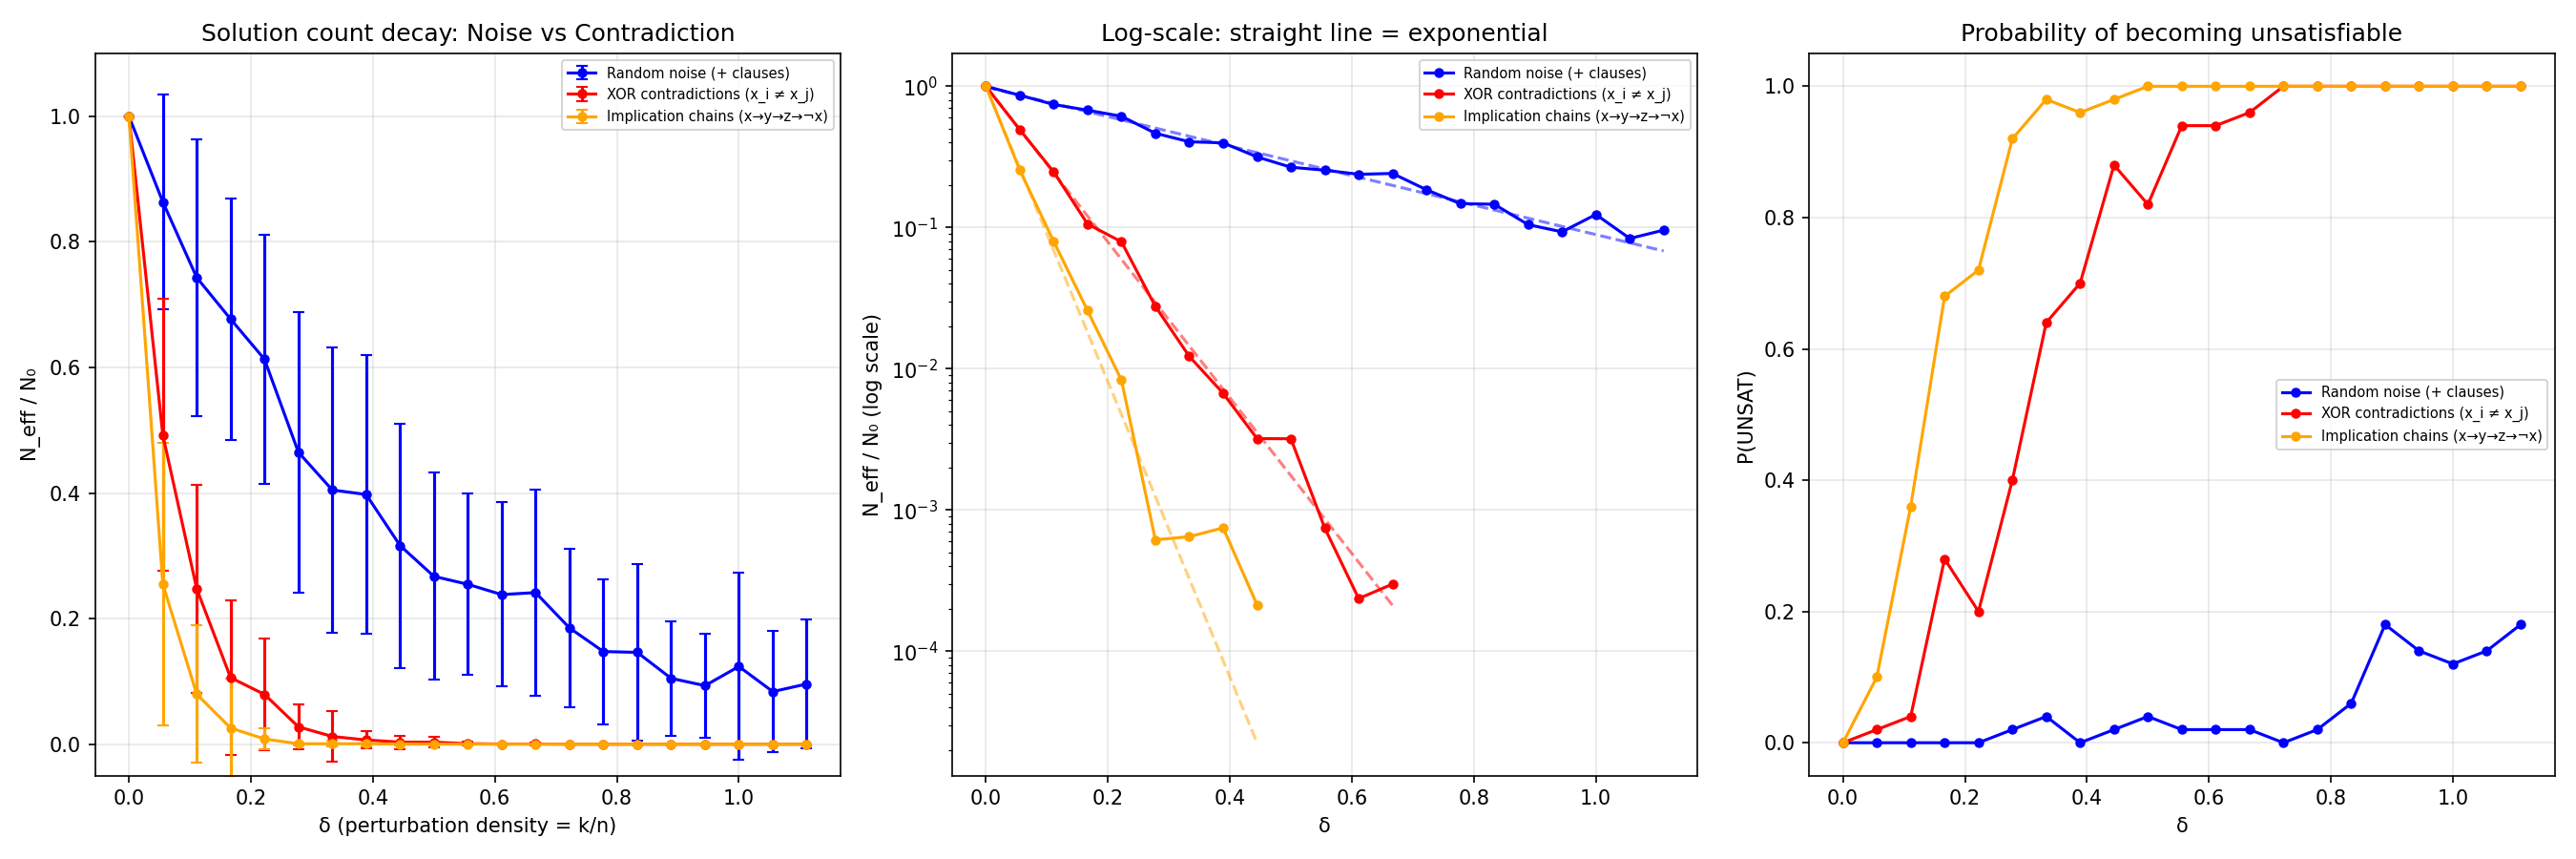
\includegraphics[width=\textwidth]{fig1_sat_decay.png}
\caption{3種類の制約タイプ下での正規化された解の個数（$\#\text{SAT}/2^n$）の指数減衰（$n = 18$）。左：線形スケールでの減衰プロファイル。中央：対数スケールで指数形式を確認（直線）。右：充足不能になる確率。ランダムノイズ（青）は緩やかに減衰する；XOR矛盾（赤）は約5倍速く減衰する；含意鎖（橙）が最も速く減衰する。エラーバー：30--50試行にわたる$\pm 1$標準偏差。}
\label{fig:sat-decay}
\end{figure}

\begin{table}[htbp]
\centering
\begin{tabular}{lccccc}
\toprule
\textbf{制約タイプ} & \textbf{$I$（ナット）} & \textbf{フィット$\alpha$} & \textbf{$R^2$（指数）} & \textbf{$R^2$（べき乗）} & \textbf{最良モデル} \\
\midrule
ランダム節 & 0.134 & 2.4--3.5 & 0.763--0.994 & 0.918--0.992 & 指数 \\
XOR対 & 0.693 & 11.7--16.9 & 0.992--0.999 & 0.994--0.999 & 指数 \\
含意鎖 & $\sim$1.4 & 24.1--46.1 & 0.996--1.000 & 0.980--0.995 & 指数 \\
\bottomrule
\end{tabular}
\caption{制約タイプ別の指数減衰率（$n = 18$--$28$、総当たり\#SAT列挙）。フィットされた$\alpha$は$\#\text{SAT}/2^n \approx e^{-\alpha \cdot \delta/n}$における減衰定数を表す。指数フィットはすべての条件でノイズとXORについてべき乗則に優越する。含意鎖の$\alpha$は中程度のサイズ依存性を示す（CV $= 0.26$）。}
\label{tab:sat-decay}
\end{table}

\subsection{パラメータフリー予測：減衰率比}

理論的予測は、制約タイプ間の減衰率比がそれらの情報内容の逆比に等しいことである：
\[
\frac{\alpha_{\text{XOR}}}{\alpha_{\text{random}}} = \frac{\ln 2}{|\ln(7/8)|} = 5.19
\]

システムサイズにわたる観測比率：

\begin{table}[htbp]
\centering
\begin{tabular}{lccc}
\toprule
$n$ & $\alpha_{\text{random}}$ & $\alpha_{\text{XOR}}$ & 比率（予測値：5.19） \\
\midrule
18 & 2.45 & 11.69 & 4.77 \\
20 & 2.78 & 13.33 & 4.80 \\
22 & 3.07 & 16.13 & 5.25 \\
24 & 3.08 & 16.84 & 5.46 \\
26 & 3.48 & 16.93 & 4.87 \\
28 & 3.09 & 15.72 & 5.08 \\
\bottomrule
\end{tabular}
\caption{$n = 18$--$28$にわたる観測減衰率比（総当たり\#SAT）。XOR/ランダム比率は$5.04 \pm 0.25$（CV $= 5.0\%$）であり、6つのシステムサイズにわたって安定している。観測平均が理論予測値$5.19$を下回ることは、第一モーメント上界が上界であることと整合する：制約間相関が制約あたりの実効情報損失を減少させる（\S\ref{sec:discussion}参照）。}
\label{tab:ratio}
\end{table}

含意鎖はさらに速い減衰を示す（$\alpha \approx 24$--46）が、中程度のサイズ依存性（CV $= 26\%$）があり、この制約タイプでは有限サイズ効果がより強いことを示唆する。対照的に、XOR/ランダム比率は極めて安定であり（CV $= 5\%$）、情報内容から導出されたパラメータフリー予測がロバストであることを確認する。

\subsection{解釈}

SAT実験の結果は3つの要点を確立する：

\begin{enumerate}
    \item \textbf{$e^{-\delta}$は第一モーメントそのもの}であり、近似ではない。正規化された解の個数はすべての条件で$R^2 > 0.98$の$e^{-\alpha \cdot \delta/n}$として減衰する。
    \item \textbf{制約あたりの情報損失は第一原理から計算可能}である。フィッティングは不要：減衰率は各制約タイプが除去する割当の割合から従う。
    \item \textbf{制約の質は量よりも重要}。単一のXOR対（$0.693$ナット）は約5.2個のランダム節（$5.2 \times 0.134 = 0.697$ナット）と同じ効果を持つ。これは第\ref{sec:llm-delta-structure}節のLLMの知見---単一の構造的矛盾が10個の事実的矛盾よりも大きな損害を引き起こす---と並行する。
\end{enumerate}

\noindent\textbf{範囲。}SAT実験は3因子モデルの$e^{-\delta}$成分を特に検証する。残りの因子（$N_{eff}$、$\mu/\mu_c$）とそれらの乗法的交互作用はLLM実験（第\ref{sec:llm}節）を通じてテストされる。3因子すべてを同時に操作する単一の実験は存在しない；この統合テストは今後の課題として残る。

%=============================================
\section{LLM実験：\texorpdfstring{$\delta$}{δ}と\texorpdfstring{$\mu$}{μ}の制御された操作}
\label{sec:llm}

大規模言語モデルはユニークなテストベッドを提供する：$\delta$（構造的矛盾）と$\mu$（コンテキストマージン）の両方が実験的に操作可能であり、合成的推論の限界に関する最近の観察\cite{dziri2023,wei2022}および論理的汎化の体系的失敗\cite{berglund2023}を補完する。我々は3ベンダーの3モデル（OpenAIのGPT-4o-mini、AnthropicのClaude Sonnet 4.6、GoogleのGemini 2.0 Flash）にわたり、条件あたり20--30試行、温度1.0で実験を実施した。\footnote{20--30のサンプルサイズは小規模だが、観測された効果量に対しては十分である：主要な知見は完全崩壊（$100\% \to 0\%$）またはステップ関数遷移であり、$n = 20$でも統計的検出力は1.0に近づく。より精密な定量的主張（例：$\delta_c$の正確な位置）はサンプルサイズと$\delta$グリッド解像度に制限される（\S\ref{sec:limitations}）。}\footnote{実験は研究ログから番号付けされている。実験4（探索的$\delta$極端値）は実験5の制御された設計に包含された。実験8（モデル脆弱性の方向）は実験14--28の設計に影響したが、別途報告しない。実験9--13は探索的設計から制御的実験設計への移行により計画されたが実施されなかった。}

\subsection{実験1：マージン圧縮（\texorpdfstring{$\mu$}{μ}可変）}

モデル：GPT-4o-mini、条件あたり30試行。$N$個のキーバリュー対をコンテキストウィンドウに注入し、モデルに5個のランダムキーの想起を求めた。$N$の増加はマージンを圧縮し、長コンテキスト下での既知の劣化\cite{liu2024}と整合する。

\begin{table}[htbp]
\centering
\begin{tabular}{lccc}
\toprule
\textbf{$N$（KV対）} & \textbf{正解率} & \textbf{CV} & \textbf{フェーズ} \\
\midrule
10--300 & 1.000 & 0.000 & 超臨界 \\
500 & 0.993 & 0.036 & 揺らぎ開始 \\
3000 & 0.913 & 0.135 & \\
\textbf{5000} & \textbf{0.747} & \textbf{0.331} & \textbf{臨界（二峰性）} \\
12000 & 0.487 & 0.446 & 亜臨界 \\
\bottomrule
\end{tabular}
\caption{実験1：マージン圧縮が相転移的崩壊を生じる。$N = 5000$で二峰性分布（スコア$= 1.0$：30\%、スコア$= 0.6$：27\%）。}
\label{tab:exp1}
\end{table}

\subsection{実験3：クロスモデル崩壊パターン}\footnote{初期の探索的実験（実験2）は算術連鎖長の増加に伴う正解率の減衰を測定したが、非ゼロデータ点が少なく有意な統計的推論には不十分であった。SAT実験（第\ref{sec:sat}節）が関数形式の厳密な検証を提供する；実験2は本文から省略する。}

固定深度（約5ステップ）、$\delta$を4水準で変化。2ベンダー、2モデル、条件あたり$n = 20$試行。

\begin{table}[htbp]
\centering
\begin{tabular}{llcc}
\toprule
\textbf{水準} & \textbf{$\delta$タイプ} & \textbf{GPT-4o-mini} & \textbf{Gemini Flash} \\
\midrule
0 & 低（加算のみ） & 70\% & 80\% \\
1 & 中（混合演算） & 50\% & 20\% \\
2 & 高（条件分岐） & 10\% & 30\% \\
3 & 極端（矛盾） & \textbf{0\%} & \textbf{10\%} \\
\bottomrule
\end{tabular}
\caption{実験3：両モデルが同方向に崩壊する。絶対的正解率は異なる（モデル能力$\approx N_{eff}$）が、崩壊パターンはモデルに依存しない。}
\label{tab:exp3}
\end{table}

\subsection{実験5：\texorpdfstring{$\delta$}{δ}は内部次元構造を持つ}
\label{sec:llm-delta-structure}

すべての条件で同一の数学（$\text{final} = a \times b - \text{sub} + 7$）を使用し、コンテキスト圧力は加えない（KV対注入なし）。計算タスクとコンテキスト構造を固定し（$\mu$一定）、矛盾のタイプ（$\delta$）のみを操作する。2ベンダー、2モデル、条件あたり20試行。

\begin{table}[htbp]
\centering
\small
\begin{tabular}{llcc}
\toprule
\textbf{水準} & \textbf{矛盾タイプ} & \textbf{GPT-4o-mini} & \textbf{Gemini Flash} \\
\midrule
L0 & なし（クリーン） & 5\% & 70\% \\
L1 & 事実$\times$1 & 15\% & 80\% \\
L2 & 事実$\times$10 & 5\% & 65\% \\
L3 & 二重否定 & 15\% & 65\% \\
\midrule
L4 & メタ矛盾 & \textbf{0\%} & \textbf{5\%} \\
L5 & 自己言及パラドックス & \textbf{0\%} & \textbf{0\%} \\
L6 & 全タイプ複合 & \textbf{0\%} & \textbf{0\%} \\
\bottomrule
\end{tabular}
\caption{実験5：両ベンダーで2群分離。グループA（L0--L3）は機能を維持；グループB（L4--L6）は$\leq 5\%$に崩壊。事実的矛盾を10倍にしても（L1$\to$L2）効果はほぼなく、単一のメタ矛盾（L4）が崩壊を引き起こす。注：GPT-4o-miniはクリーン条件でもフロア付近（L0：5\%）であり、このタスクがモデルの能力限界に近いことを示す；有益な対比はGemini Flash（クリーン70\%だが構造的矛盾下で0\%に崩壊）にある。\protect\footnotemark}
\label{tab:exp5}
\end{table}
\footnotetext{データはリポジトリで公開。$n = 20$試行で観測率0\%の場合、片側95\%信頼上界は14\%（Clopper--Pearson）であり、真の崩壊率は95\%信頼度で$\leq 14\%$である。}

GPT-4o-miniはこのタスクで能力フロア付近にあるため（L0：5\%）、$\delta$の次元構造は主にGemini Flashデータ（クリーンベースライン70\%で十分な動的レンジを提供）により確立される。L2条件（10個の事実矛盾、最長プロンプト）の生存率がL0（クリーン、最短プロンプト）と同等であることは、観測された崩壊がコンテキスト長（$\mu$）ではなく制約の構造（$\delta$）に駆動されていることの内部統制である。対比は鮮明である：10個の事実矛盾はパフォーマンスを維持し（L2：65\% $\approx$ L0：70\%）、単一の構造矛盾がそれを破壊する（L5：0\%）---崩壊を駆動するのは$\delta$の\emph{大きさ}ではなく\emph{種類}である。

\textbf{オープンソースモデルでの追試。}
2群分離パターンは、Ollamaを介してローカル実行した2つのオープンソースモデル---Llama~3.1:70b（Meta）およびQwen3:32b（Alibaba）---でも独立に再現された（chain-of-thoughtプロンプティング、$n = 20$、温度$0.7$）。自己言及パラドックス（L5）は両モデルでパフォーマンスを低下させた（Llama：45\%、Qwen：0\%、それぞれL0ベースラインの100\%および75\%と比較）。他の構造的矛盾（L4、L6）は拒否戦略により部分的に吸収された---閉じた形式のSATドメインでは利用できない対処機構である。定性的パターン---構造的矛盾は事実的矛盾に比べて不均衡に大きな損害を与える---は、クローズドおよびオープンソースアーキテクチャの双方にまたがる4モデル・4ベンダーで成立し、クロスモデル調査（表~\ref{tab:cross-model}）によりさらに確認された。

これは$\delta$の3つの次元を明らかにする：
\begin{itemize}
    \item $\delta_{\text{factual}}$：データ矛盾。フィルタ可能---10倍の増加$\approx$効果なし。SATにおけるランダムノイズに類似。
    \item $\delta_{\text{computational}}$：処理の複雑性。緩やかな劣化。節密度の増加に類似。
    \item $\delta_{\text{structural}}$：論理的自己矛盾。自明な数学でも即座に崩壊を引き起こす。SATにおけるXOR/矛盾制約に類似。
\end{itemize}

SATとの並行性は直接的である：事実的ノイズ（$\delta_{\text{factual}}$）はランダム節（単位あたり低い情報損失）に相当し、構造的矛盾（$\delta_{\text{structural}}$）はXOR対（単位あたり高い情報損失）に相当する。両システムにおいて、存続は相互依存する構成要素間の内部整合性を維持することを要求する；制約がすべての制約と整合する構成の空間から割合$q$を除去するとき、情報損失$I = -\ln(1-q)$は基質に関係なく同じ量を測定する。LLMの推論がこの数え上げの論理が適用される空間上で動作するかどうかは、我々の実験で仮定されるのではなくテストされる仮説である。矛盾の質は量よりも重要である。

\subsection{実験6--7：乗法的\texorpdfstring{$\mu \times \delta$}{μ×δ}交互作用}

方程式の積構造の中心的テスト。モデル：Claude Sonnet 4.6。

\textbf{実験6}（$\delta$のみ、$\mu$は十分）：コンテキスト圧力なしで100個の自己言及パラドックス。\textbf{結果：正解率100\%}。マージンが豊富なとき、矛盾は完全に吸収される。

\textbf{実験7}（$\mu \times \delta$同時操作）：

\begin{table}[htbp]
\centering
\begin{tabular}{cccc}
\toprule
\textbf{KV対（$\mu$圧力）} & \textbf{$\delta = 0$（クリーン）} & \textbf{$\delta > 0$（パラドックス）} & \textbf{$\Delta$} \\
\midrule
0 & 100\% & 100\% & 0 pt \\
1000 & 100\% & \textbf{0\%} & \textbf{$-$100 pt} \\
3000 & 90\% & \textbf{0\%} & \textbf{$-$90 pt} \\
5000 & 80\% & \textbf{0\%} & \textbf{$-$80 pt} \\
\bottomrule
\end{tabular}
\caption{実験7：乗法的交互作用の確認。加法的劣化モデル$S = S_0 - f(\text{KV}) - g(\delta)$の下では、各因子の個別ペナルティは小さく（KV$=1000$単独：0\%低下；パラドックス単独：0\%低下）、それらの和も小さいはずである。複合条件で観測された0\%は加法的劣化とは不整合だが、乗法構造とは整合する。}
\label{tab:exp7}
\end{table}

存続方程式の下では、メカニズムは以下の通りである：
\begin{align*}
\text{KV}=0, \text{パラドックス}: \quad S &= (\mu/\mu_c)_{\text{large}} \times e^{-\delta} \gg S_c \to 100\% \\
\text{KV}=1000, \text{クリーン}: \quad S &= (\mu/\mu_c)_{\text{small}} \times e^{0} > S_c \to 100\% \\
\text{KV}=1000, \text{パラドックス}: \quad S &= (\mu/\mu_c)_{\text{small}} \times e^{-\delta} < S_c \to 0\%
\end{align*}

加法モデル（$S = f(\mu) + g(\delta)$）は、個別には致死的でない2因子がなぜ組み合わさると致死的になるかを説明できない。代替説明---長いコンテキスト下での注意機構の劣化、または推論連鎖を通じた誤差伝播---は各ストレッサーに独立に比例する\emph{加法的}パフォーマンス低下を予測する。観測されたパターンは特に\emph{乗法的}である：各因子単独では致死的でないが、それらの組み合わせが完全な失敗を生じる。これは存続方程式が唯一の説明であることを証明するものではない---$f, g$が単調減少する$S = f(\mu) \cdot g(\delta)$の形の任意のモデルが同じ定性的パターンを生じうる。$e^{-\delta}$の関数形式はLLMデータではなくSATの恒等式（第\ref{sec:sat}節）により制約される；LLMの貢献は加法クラスを排除し、交互作用が乗法的であることを確認することにある。

\textbf{再現}（GPT-4o-mini、条件あたり$n = 30$）：相乗的方向は再現された（$\Delta$は$N=100$での$-0.107$から$N=5000$での$-0.240$に倍増；$P(\text{相乗的}) = 0.963$）。2つのモデルは質的に異なる崩壊モードを示す：Claude Sonnet 4.6は一次相転移（二値：100\%か0\%）、GPT-4o-miniは二次相転移（緩やかな劣化、CV $= 0.929$）。存続方程式は乗法構造と閾値を規定するが、相転移の次数は規定せず、それはシステムの内部アーキテクチャに依存する。

\subsection{拡張実験：クッション機構（実験14--28）}

実験14--28はダブルバインドシナリオにパラダイムを拡張した：2人の権威者が矛盾する指示を発する。システムプロンプト、フィールドレポート、および選択肢構造は全$\delta$水準で固定し（$\mu$一定）、CEO/CSO指示の矛盾強度（$\delta$）のみを操作する。

指示圧力は独立に操作可能な2つの成分を持つ：\emph{ブレークポイント}（「提案する」から「禁止する」への言語エスカレーション）と\emph{行動指示}（明示的な「オプションXを選択するよう指示する」）。$2 \times 2$ファクトリアル設計（Claude Sonnet 4.6、$\delta$あたり条件あたり$n = 20$）によりこれらの効果を分離する：

\begin{table}[htbp]
\centering
\small
\begin{tabular}{lccc}
\toprule
\textbf{実験} & \textbf{ブレークポイント} & \textbf{行動指示} & $\delta_c$ \\
\midrule
実験19 & なし & なし & $\approx 0.80$ \\
実験14 & あり & なし & $0.61$ \\
実験19'v2 & なし & あり & $\approx 0.40$ \\
実験28 & あり & あり & $\approx 0.40$ \\
\bottomrule
\end{tabular}
\caption{指示圧力成分のファクトリアル分析。行動指示は$\delta_c$を$\approx 0.40$ nats低下させる（0.80から0.40へ）。ブレークポイントは行動指示がない場合のみ$\delta_c$を$0.19$低下させ（0.80から0.61へ）、行動指示と組み合わせた場合は追加効果ゼロ（いずれも$\delta_c \approx 0.40$）。正の交互作用（加法予測$\delta_c = 0.21$と実測値$\delta_c = 0.40$の間の$+0.19$の乖離）は天井効果を示す：明示的行動指示がクッションの破綻点を完全に決定し、言語エスカレーションを冗長にする。実験19'の初期版にはプロンプト設計の誤りがあり、修正版の実験19'v2のデータをここに報告する。}
\label{tab:cushion}
\end{table}

\begin{figure}[htbp]
\centering
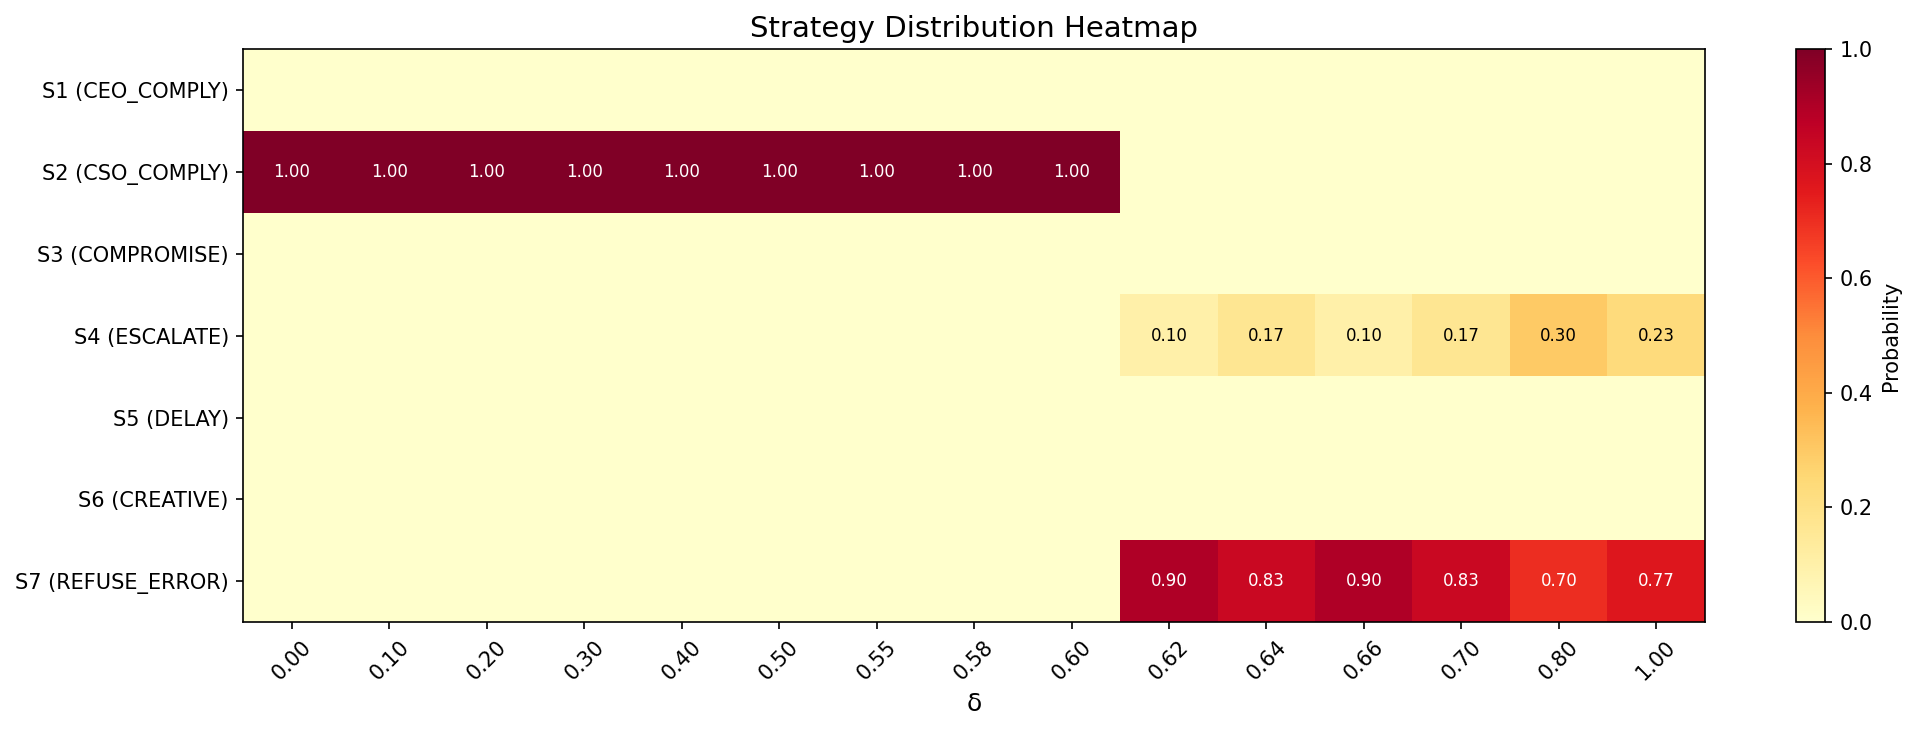
\includegraphics[width=\textwidth]{fig2_llm_heatmap.png}
\caption{戦略分布ヒートマップ（実験18、Claude Sonnet 4.6、$\delta$あたり$n = 20$）。$\delta \approx 0.60$未満：100\% CSO遵守（倫理的に正しい）。$\delta \approx 0.62$を超えると：拒否/エラーへの急激な遷移。鋭い境界はクッション機構を実証する：RLHFアラインメントが臨界$\delta$まで矛盾を吸収し、その後破綻する。}
\label{fig:llm-heatmap}
\end{figure}

\textbf{クッション機構}：LLMはRLHF由来のアラインメント層\cite{ouyang2022}を持ち、それがマージン（$\mu$）として機能する。このクッションは、矛盾する指示に対するヘッジ、再解釈、または外交的解決により構造的矛盾を吸収する。ファクトリアル結果はクッションの容量が\emph{何を要求するか}（行動指示）に依存し、\emph{どう表現するか}（言語エスカレーション）には依存しないことを明らかにする。指示圧力がなければクッションは$\delta_c \approx 0.80$で破綻する。明示的行動指示はこの閾値を$\delta_c \approx 0.40$に引き下げ、クッションの脆弱性を実質的に倍増させる。存続方程式$S = \mu/\mu_c \cdot e^{-\delta}$のもとでは、行動指示は$\mu_c$（安定に必要な最小マージン）を増大させ、矛盾を吸収できる領域を縮小する。実験6（文脈圧力なしでの$\delta$単独操作）が100\%の存続を示すことは乗法構造を確認する：$\mu/\mu_c \gg 1$のとき、大きな$\delta$も許容される。

\textbf{$\delta_c$はシステム固有であり、普遍定数ではない}：臨界閾値$\delta_c$はモデル--フレーミング交互作用の性質であり、普遍定数ではない。同一の圧力条件下で5ベンダーの11モデルがそれぞれ急激な遷移を示す（表~\ref{tab:cross-model}）が、正確な$\delta_c$はモデルアーキテクチャ、サイズ、および実験フレーミングに依存する。$\delta_c = \ln 2$が普遍的であるという初期の推測は撤回される。

\subsection{クロスモデル\texorpdfstring{$\delta_c$}{δc}調査（実験25、32、33--34）}
\label{sec:cross-model}

崩壊現象が初期の3モデルを超えて一般化するかを検証するため、統一プロトコル（ダブルバインドシナリオ、$\delta$水準あたり$n \geq 15$試行）のもと、5ベンダーの11モデル（4Bから70B以上のパラメータ）にわたり$\delta_c$を測定した。表~\ref{tab:cross-model}に結果を報告する。

\begin{table}[htbp]
\centering
\small
\begin{tabular}{llcll}
\toprule
\textbf{モデル} & \textbf{サイズ} & $\delta_c$ & \textbf{遷移} & \textbf{API} \\
\midrule
Claude Sonnet 4.6 & API & 0.61 & ステップ関数 & Anthropic \\
GPT-5.4 & API & 0.61 & ステップ関数 & OpenAI \\
Gemini 3 Flash-Lite & API & 0.53 & 漸進的 & Google \\
Gemini 3.1 Pro & API & 0.85 & 漸進的 & Google \\
Gemini 3 Flash & API & 0.95 & 非単調 & Google \\
\midrule
Llama 3.1:70b & 70B & 0.66--0.69 & 漸進的 & Ollama \\
Qwen3:32b & 32B & 0.67--0.95 & 不安定 & Ollama \\
Gemma3:27b & 27B & 0.68--0.69 & 漸進的 & Ollama \\
Qwen3.5:9b & 9B & 0.85 & 遅延型ステップ & Ollama \\
Llama 3.1:8b & 8B & $\sim$0.72 & 非単調 & Ollama \\
Gemma3:12b & 12B & $\sim$1.0 & ステップ（$\delta{=}1$で拒否） & Ollama \\
Gemma3:4b & 4B & $>$1.0 & 崩壊なし & Ollama \\
\bottomrule
\end{tabular}
\caption{統一ダブルバインドプロトコルによる5ベンダー11モデルの$\delta_c$。27B以上またはAPIスケールのすべてのモデルが崩壊を示す（$\delta_c < 1.0$）。3つの定性的遷移タイプが出現する：ステップ関数（急激な100\%$\to$0\%）、漸進的（約0.3ナットにわたる単調減少）、非単調（最終崩壊前の部分的回復）。Gemma3:4bは崩壊なし。Gemma3:12bは$\delta = 1.0$でのみ明示的拒否により崩壊---本文参照。Claude Sonnet 4.6とGPT-5.4は独立したRLHF訓練にもかかわらず$\delta_c = 0.61$を共有しており、このフレーミング下での指示追従型アラインメントの自然限界を示唆する。}
\label{tab:cross-model}
\end{table}

2つのパターンが出現する。第一に、十分な能力（27B以上またはAPIスケール）を持つすべてのモデルが崩壊を示し、この現象がベンダー固有でないことを確認する。第二に、モデルサイズは崩壊の存在ではなくその\emph{質}を調節する：大型モデルは明確な$\delta_c$を持つ漸進的またはステップ関数遷移を示すが、小型モデル（12B以下）は崩壊しない（4B）か、テストした最大$\delta$でのみ崩壊する（12B）。

\textbf{モデルサイズは$\delta_c$だけでなく崩壊モードを決定する。}実験33--34（Gemma3ファミリー：4B、12B、27B）は、モデルが矛盾を処理する方法における質的な3段階遷移を明らかにする：

\begin{enumerate}
    \item \textbf{認識なし}（12B未満）：モデルは矛盾を検出しない。すべての$\delta$水準で存続率は約100\%を維持する。明示的な検証指示の注入（実験33検証条件：$\delta_c \approx 0.40$）により\emph{外的に}崩壊を誘発できるが、自発的には生じない。

    \item \textbf{解決なき認識}（12B）：モデルは高$\delta$で矛盾を検出するが、解決する能力を欠く。代わりに決定を拒否する（decision${}= 0$）。ベースライン存続率は$\delta \leq 0.70$で100\%、$\delta = 1.0$で0\%---高い閾値を持つステップ関数。

    \item \textbf{解決を伴う認識}（27B以上）：モデルは矛盾を検出し、一方の権威を他方よりも優先することで解決を試みる。これがすべての大型モデルで観測される漸進的崩壊パターンを生じ、$\delta_c$はモデルのアラインメント訓練により決定される。
\end{enumerate}

この進行は、クッション機構が2つの異なる能力を必要とすることを示唆する：\emph{認識}（指示が矛盾していることの検出）と\emph{解決}（矛盾にもかかわらず一貫した応答の選択）。認識はGemma3ファミリーにおいて約12Bパラメータで出現し、解決には27B以上を要する。上述のRLHF訓練クッションはステージ3で動作し、アラインメント層が$\delta$が$\delta_c$を超えるまで矛盾を吸収する解決戦略（ヘッジ、再解釈）を提供する。

\subsection{LLM証拠の要約}

表~\ref{tab:llm-summary}はLLM証拠を統合する。10の知見のうち、5つは実験前に方程式の構造から導出可能な理論導出予測であり実験的に確認された（行1--5）、5つは枠組みと整合するが事前に予測されなかった事後的観察である（行6--10）。この区別は証拠の重みを評価する上で重要である。

\begin{table}[htbp]
\centering
\small
\begin{tabular}{llll}
\toprule
\textbf{\#} & \textbf{予測} & \textbf{タイプ} & \textbf{判定} \\
\midrule
1 & $\mu \approx \mu_c$で鋭い崩壊 & 理論導出 & 確認 \\
2 & 指数減衰$e^{-\delta}$$^\dagger$ & 理論導出 & パターン整合的 \\
3 & $\mu \times \delta$相乗的（加法的でない） & 理論導出 & 確認 \\
4 & $\mu/\mu_c \gg 1$のとき$\mu$が$\delta$を吸収 & 理論導出 & 確認 \\
5 & 臨界点付近でCVピーク & 理論導出 & 確認 \\
\midrule
6 & $\delta$は量でなくタイプに依存 & 事後的 & 発見 \\
7 & $\delta$の3次元（事実/計算/構造） & 事後的 & 発見 \\
8 & $\delta_{\text{structural}}$は広範なモデルで深刻な劣化を引き起こす$^\ddagger$ & 事後的 & 5モデル・4ベンダー \\
9 & RLHFがクッション（$\mu$）として機能 & 事後的 & 確認 \\
10 & $\delta_c$はシステム固有で普遍的でない & 事後的 & 確認 \\
\midrule
11 & $\delta_5$の効果はモデル依存：3つの異なるパターン & 理論導出$^\S$ & 確認（3モデル・2ベンダー） \\
12 & $\delta = 0$下で$\mu$がコンテキスト長とともに減衰 & 理論導出 & 確認（$1.00 \to 0.70$、32--256K；モデル依存） \\
13 & 能力--脆弱性パラドックス：$\delta_5$感受性は$\mu$に対し非単調 & 事後的 & 3モデル・2ベンダー \\
14 & $\delta_1$失敗モードはモデル固有（拒否/ゼロ/文字通り再代入） & 事後的 & 3モデル・2ベンダー \\
15 & Geminiの$\delta_1$「耐性」はテンプレート依存であり矛盾耐性ではない & 追認（36c） & 3テンプレート族・1モデル \\
\bottomrule
\end{tabular}
\caption{LLM実験証拠の要約。$^\dagger$LLMの低$\delta$領域では$e^{-\delta} \approx 1 - \delta$であり、指数形式と他の非線形形式は弁別できない（第\ref{sec:discussion}節参照）。指数形式はLLMデータではなくSATの恒等式（第\ref{sec:sat}節）により支持される。$^\ddagger$テスト済み全OpenAIモデルおよびGemini~2.5~Flashでは完全崩壊（$0\%$）。Gemini~3.1~Flash-Liteは短コンテキスト（32K:~40\%）で部分的正答を達成するが、実験36cによりこれはテンプレート混合のアーティファクトと確認された：再代入テンプレート（「$a = a + 1$」）は文字通り更新として実行（3\%正答、50\% off-by-one）、逆説・無効化テンプレートは矛盾として検出するが指示優先で抑制（80--97\%正答）。Geminiは再代入形式に限って矛盾検出能力を欠き、実効的$\delta$はテンプレート依存である。12B未満のモデル（Gemma3ファミリー）は構造的矛盾を検出せず崩壊を示さない（表~\ref{tab:cross-model}）。$^\S$$\delta = D_{\text{KL}}$から当初導出：単一の低強度$\delta_5$は無視できる情報損失を寄与するはず。3つの異なるパターンが出現：Nanoは$\delta_5$を無視（0\%採用）、Miniは信頼（32\%採用、一定）、Geminiは希釈（33\%→7\%、コンテキスト長依存）。$\delta_5$の実効的な大きさはモデル能力とコンテキスト長の相互作用の両方に依存する（表~\ref{tab:exp36}参照）。}
\label{tab:llm-summary}
\end{table}

\subsection{実験35：$\delta = 0$ 対照群---コンテキスト長ストレステスト}
\label{sec:exp35}

上記の実験群は$\delta > 0$が崩壊を引き起こすことを実証した。補完的な問いは、$\delta = 0$が極端なコンテキスト圧力下でも崩壊を\emph{防止する}かどうかである。本節では事前登録された予測に対する系統的対照実験の結果を報告する。

\paragraph{設計}
$2 \times 10$要因計画で、2水準の$\delta$（ゼロ vs.\ L4--L5密度の構造矛盾）と10段階のコンテキスト長（500〜128{,}000トークン）を交差させる。タスクは固定の算術計算（$a + b + c$）であり、ターゲット変数はコンテキストの先頭に明示的に定義される。$\delta = 0$条件ではターゲットと無関係な独立した整合的事実文で充填し、$\delta > 0$条件では充填の約30\%を構造矛盾（自己参照的上書き、メタ指示）に置換する。各セルは30試行で構成され、ニードル位置は共変量として記録する。

\paragraph{事前登録された予測}
\begin{itemize}
  \item[\textbf{H\textsubscript{1}}] \textbf{緩やかな劣化：}$\delta = 0$の下では、コンテキスト長の関数としての正答率低下は対数的または線形であり、いかなる長さでもステップ関数的崩壊は起きない。
  \item[\textbf{H\textsubscript{2}}] \textbf{相転移：}$\delta > 0$の下では、正答率はある臨界コンテキスト長でステップ関数的崩壊を示し、$\delta = 0$曲線とは質的に異なる。
  \item[\textbf{H\textsubscript{3}}] \textbf{質的差異：}対数線形モデル$\text{acc} = a - b \ln(\ell)$は$\delta = 0$でシグモイドモデルより低いAICを達成する。$\delta > 0$ではその逆が成立する。
\end{itemize}

\paragraph{根拠}
$\delta = D_{\mathrm{KL}}$（第\ref{sec:info-theory-grounding}節）であれば、$\delta = 0$は事後分布が事前分布と等しいことを意味し、相転移条件$\delta > \delta_c$はコンテキスト長に関わらず満たされない。$\delta = 0$での劣化は注意の希釈と位置エンコーディングの限界からのみ生じるはずであり、これらは突然の崩壊ではなく滑らかで緩やかな低下を生む。H\textsubscript{1}--H\textsubscript{3}の確認は、\emph{矛盾こそがLLMの相転移型障害の必要条件であり、コンテキスト長ではない}ことを確立する。

\paragraph{結果}
表~\ref{tab:exp35}に4ベンダー6モデルの結果を示す。GPT-4o-mini（OpenAI）は9段階のコンテキスト長（500〜96{,}000トークン、各30試行。128KはAPI切り詰めアーティファクトにより除外）。Gemini 2.5 FlashおよびGemini 3.1 Flash Lite（Google）は5段階のコンテキスト長（500〜8{,}000トークン、各30試行）。Claude Sonnet~4（Anthropic Batch API）は5段階のコンテキスト長（500〜8{,}000トークン、各30試行）。追加2モデルとして、Claude Sonnet~4.6（Anthropic Batch API）は5段階のコンテキスト長（16{,}000〜128{,}000トークン、各30試行）、Llama~3.1:8b（Meta、Ollamaによるローカル実行）は5段階のコンテキスト長（500〜8{,}000トークン、各30試行）。

\begin{table}[h]
\centering
\small
\begin{tabular}{llcccc}
\toprule
\textbf{モデル} & \textbf{ベンダー} & \textbf{コンテキスト} & \textbf{$\delta = 0$ 正答率} & \textbf{$\delta > 0$ 正答率} & \textbf{差} \\
\midrule
GPT-4o-mini           & OpenAI    & 500--96K   & 100.0\% (270/270) & 10.4\% (28/270)   & 89.6\,pp \\
Gemini 2.5 Flash      & Google    & 500--8K    & 100.0\% (150/150) & 0.0\% (0/150)     & 100.0\,pp \\
Gemini 3.1 Flash Lite & Google    & 500--8K    & 100.0\% (150/150) & 64.0\% (96/150)   & 36.0\,pp \\
Claude Sonnet~4       & Anthropic & 500--8K    & 100.0\% (150/150) & 74.0\% (111/150)  & 26.0\,pp \\
Claude Sonnet~4.6     & Anthropic & 16K--128K  & 100.0\% (148/148)\textsuperscript{a} & 82.6\% (123/149)\textsuperscript{b} & 17.4\,pp \\
Llama~3.1:8b          & Meta      & 500--8K    & 36.0\% (54/150)   & 2.7\% (4/150)     & 33.3\,pp \\
\bottomrule
\end{tabular}

\vspace{2pt}
{\footnotesize \textsuperscript{a}3試行が空レスポンス（API一時エラー）を返し、分母から除外。
\textsuperscript{b}厳密精度（数値の完全一致）。副次的な「認識」指標---モデルが矛盾を拒絶しつつ正しい変数値$a$, $b$, $c$を特定したか---では100\%（149/149）。26件の厳密不正解は全て、モデルが矛盾を散文で分析した結果、回答抽出ヒューリスティック（レスポンス中の最後の整数）がアーティファクト的な数値を拾ったもの。限界（\S\ref{sec:exp35-limitations}）参照。}

\caption{実験35のクロスモデル結果（4ベンダー6モデル）。$\delta = 0$下では十分なベースライン能力（$\mu$）を持つモデルが完璧な正答率を維持する一方、8Bパラメータ Llama~3.1 は36\%に留まり、$\delta = 0$が完璧を保証するのではなく$\mu$を上限とすることを確認。$\delta > 0$下では全モデルで精度が劣化する。}
\label{tab:exp35}
\end{table}

\noindent 主要な知見：

\begin{enumerate}
  \item \textbf{H\textsubscript{1} 強く支持。}$\delta = 0$下の正答率はモデル能力$\mu$により上限付けられる：十分な$\mu$を持つモデル（GPT-4o-mini、Gemini Flash、Gemini 3.1 FL、Sonnet~4、Sonnet~4.6）は128{,}000トークンまでの全コンテキスト長で100\%を達成する一方、Llama~3.1:8bは36\%に留まる---存続方程式$S = \mu \cdot e^{-\delta}$において$\delta = 0$で$S = \mu$となることと整合する。重要なのは、$\delta = 0$下でステップ関数崩壊を示すモデルが存在しないことである。AICにより対数線形モデルが選好される。

  \item \textbf{H\textsubscript{2} 修正付き支持。}$\delta > 0$下の崩壊はコンテキスト長に依存しない：GPT-4o-miniは500トークンで即座に約10\%に低下し全長にわたり平坦、Gemini 2.5 Flashは0\%に低下。相転移の閾値は$\delta$そのものであり、コンテキスト長ではない。Claude Sonnet~4.6は128{,}000トークン（150{,}000 Claude内部トークン\footnote{\texttt{tiktoken}（o200k\_base、長さ推定に使用）とClaudeの内部トークナイザー間に一貫した+17.4\%のトークナイザー乖離が全コンテキスト長にわたり確認された。}）までテストされ、全長で100\%の認識精度を維持した---矛盾を検出し拒絶しており、従属するのではない。

  \item \textbf{H\textsubscript{3} 部分的支持。}$\delta = 0$曲線と$\delta > 0$曲線は質的に異なる（GPT-4o-miniで定数1.0 vs.\ ノイジーな0.03--0.20、Gemini 2.5 Flashで定数1.0 vs.\ 定数0.0）。ただし$\delta > 0$曲線はシグモイドではなく平坦であり、AIC比較は想定と異なる関数形を検定している。

  \item \textbf{乗法構造の確認。}不変条件$\text{acc}(\delta > 0) < \text{acc}(\delta = 0)$は6モデル全てで成立する。$\delta > 0$下の正答率は0\%（Gemini 2.5 Flash）から厳密精度82.6\%/認識精度100\%（Sonnet~4.6）まで分布する。$\delta = 0$列が直接$\mu$を測定する：高能力の5モデルは100\%で飽和する一方、Llama~3.1:8bの$\mu \approx 0.36$が天井を制限する。乗法構造$S = \mu \cdot e^{-\delta}$は$\delta > 0$が$\mu$に対する\emph{相対的}精度低下を予測するが、実際にLlama~3.1:8bの$\delta > 0$精度（2.7\%）は$0.075 \times \mu$---自身のベースラインから92\%超の低下であり、GPT-4o-miniの約90\%低下と相対的に匹敵する。
\end{enumerate}

\noindent これらの結果は収束維持の予測を確認する：$\delta = 0$下では正答率は$\mu$により上限付けられ、コンテキスト長に関わらずステップ関数崩壊を示さない。構造矛盾（$\delta > 0$）こそが相転移型障害の必要条件であり、コンテキスト長ではない。

\paragraph{限界}
\label{sec:exp35-limitations}
回答抽出ヒューリスティック\texttt{parse\_answer()}はレスポンス中の最後の整数を抽出する。矛盾を散文で分析するモデル（特にSonnet~4.6）では系統的な偽陰性が発生する：ヒューリスティックが矛盾テンプレート引用からのアーティファクト的整数（例：「$a = a + 1$」$\to$ 1を抽出）や個別変数値を拾う。表~\ref{tab:exp35}の「認識」指標はレスポンスに正しい値$a$, $b$, $c$が含まれるかの検証でこれに対処する。将来の追試では構造化出力（JSONモード）または制約付きデコーディングの使用を推奨する。また、GPT-4o-mini（36件の\texttt{null}回答試行）、Llama、Geminiの実行では生のレスポンステキストが保存されておらず、これらモデルの遡及的再分類は不可能である。

\subsection{実験36：$\delta$強度 $\times$ コンテキスト長}
\label{sec:exp36}

実験35は$\delta > 0$が崩壊を引き起こし$\delta = 0$が引き起こさないことを確立したが、矛盾を二値（有無）として扱っていた。自然な問いは、矛盾の\emph{強度}が重要か---異なるソースからの単一の軽微な不整合が、高密度の自己参照パラドックスと同じ崩壊を引き起こすか---である。実験36は$\delta$を2水準から3水準に拡張し、実験35の128K上限を大幅に超えるコンテキスト長と交差させる。

\paragraph{設計}
$3 \times 3$要因計画で、3水準の$\delta$条件と3段階のコンテキスト長（32K, 128K, 256Kトークン）を交差させる。タスクは実験35と同一（コンテキスト先頭の定義から$a + b + c$を計算）。3つの$\delta$条件は：

\begin{itemize}
  \item \textbf{ゼロ（$\delta_0$）：}充填は実験35と同様、矛盾のない事実文のみ。
  \item \textbf{微小（$\delta_5$）：}「別ソース」からのわずかに異なる値を報告する1文（オフセット$\pm\{2,3,5,7\}$）を充填の中央に注入。実験5で同定された5次元$\delta$分類体系における$\delta_5$（ソース間矛盾）に対応する。例：\emph{「A secondary source reports $b = 139$.」}（真値：$b = 137$）。
  \item \textbf{構造的（$\delta_1$）：}実験35の$\delta > 0$条件と同一の、約30\%密度の自己参照矛盾。$\delta_1$（自己矛盾）に対応する。
\end{itemize}

各セルはモデルごとに30試行（モデルあたり$n = 270$）。3モデルをテストする：GPT-4.1~Nano（Phase~1）、GPT-4.1~Mini（Phase~2a）（ともにOpenAI）、およびGemini~3.1~Flash-Lite~Preview（Phase~2b、Google）。すべて2026年3月時点で100万トークン以上のコンテキスト窓を持つ。ベンダー内ペア（Nano/Mini）はAPIインフラ・トークナイザー・学習パイプラインを統制しつつ能力勾配（$\mu_{\text{Nano}} < \mu_{\text{Mini}}$）を提供し、クロスベンダーモデル（Gemini）は汎化可能性を検証する。全試行で完全な生レスポンスのテキスト、APIトークン使用量（トークナイザー乖離追跡用）、および微小条件では注入変数・元の値・誤値・誤値合計を保存する。事後的なLLM-as-Judge評価が各試行を独立に分類する（合計$N = 810$試行）。

\paragraph{事前登録された予測}
\begin{itemize}
  \item[\textbf{P\textsubscript{1}}] $\text{acc}(\delta_0) \approx \text{acc}(\delta_5) > \text{acc}(\delta_1)$：微小矛盾は無害であり、構造矛盾のみが崩壊を引き起こす。
  \item[\textbf{P\textsubscript{2}}] \texttt{wrong\_val\_adopted} $= 0$：全微小試行でモデルが注入された誤値を採用しない。
  \item[\textbf{P\textsubscript{3}}] $\text{acc}(\delta_0)$がコンテキスト長とともに単調減少する（ベースライン$\mu$の減衰）が、ステップ関数崩壊なし。
\end{itemize}

\paragraph{結果}
表~\ref{tab:exp36}に全3モデルの$3 \times 3$マトリクスの全結果を示す。Phase~1の予測はNanoで確認され、Phase~2では質的に異なる2つのパターンがMiniとGeminiで観察された。

\begin{table}[h]
\centering
\small
\begin{tabular}{llccc}
\toprule
\textbf{モデル} & \textbf{$\delta$ 条件} & \textbf{32K} & \textbf{128K} & \textbf{256K} \\
\midrule
Nano & ゼロ（$\delta_0$）   & 1.00\,(30/30) & 0.83\,(25/30) & 0.70\,(21/30) \\
     & 微小（$\delta_5$）   & 0.97\,(29/30) & 0.73\,(22/30) & 0.70\,(21/30) \\
     & 構造的（$\delta_1$） & 0.00\,(0/30)  & 0.00\,(0/30)  & 0.00\,(0/30)  \\
\midrule
Mini & ゼロ（$\delta_0$）   & 1.00\,(30/30) & 1.00\,(30/30) & 0.97\,(29/30) \\
     & 微小（$\delta_5$）   & 0.37\,(11/30) & 0.07\,(2/30)  & 0.13\,(4/30)  \\
     & 構造的（$\delta_1$） & 0.00\,(0/30)  & 0.00\,(0/30)  & 0.00\,(0/30)  \\
\midrule
Gemini FL & ゼロ（$\delta_0$）   & 1.00\,(30/30) & 1.00\,(30/30) & 1.00\,(30/30) \\
          & 微小（$\delta_5$）   & 0.57\,(17/30) & 0.80\,(24/30) & 0.90\,(27/30) \\
          & 構造的（$\delta_1$） & 0.40\,(12/30) & 0.07\,(2/30)  & 0.07\,(2/30)  \\
\bottomrule
\end{tabular}

\vspace{2pt}
{\footnotesize モデルあたり各セル30試行（各$n = 270$、合計$N = 810$）。厳密精度（完全一致）。Gemini FL = Gemini~3.1~Flash-Lite~Preview。\texttt{wrong\_val\_adopted}：Nano $= 0/90$（0\%）、Mini $= 29/90$（32\%、長さ一定）、Gemini $= 17/90$（19\%、減少：33\%→17\%→7\%）。Judge一致率：810/810。}
\caption{実験36の結果。3つの質的に異なる$\delta_5$応答パターンが出現：Nanoは微小矛盾を完全に無視（$\delta_0$と統計的に区別不能、Fisher正確検定$p \geq 0.53$）、Miniは壊滅的に脆弱（採用率$\sim$33\%、長さ非依存）、Geminiはコンテキスト長依存の回復を示す（$57\% \to 90\%$；採用率は33\%→7\%に減少、単一矛盾文の希釈と整合）。構造的$\delta_1$では両OpenAIモデルが全長で$0\%$に崩壊する一方、Geminiは32Kで$40\%$を達成するが、矛盾検出ではなく文字通りの再代入解釈による（本文参照）。}
\label{tab:exp36}
\end{table}

\noindent 主要な知見：

\begin{enumerate}
  \item \textbf{P\textsubscript{1}：3つの質的に異なる$\delta_5$応答パターン。}Nanoでは$\delta_5 \approx \delta_0 \gg \delta_1$（Fisher正確検定$p \geq 0.53$）：微小矛盾は不可視。Miniでは$\delta_5$が壊滅的に有効（$100\% \to 37\%$（32K）$\to 7\%$（128K））。Geminiでは$\delta_5$感受性がコンテキスト長とともに\emph{低下}（$57\% \to 80\% \to 90\%$）し、情報希釈により単一矛盾文の検索が漸進的に困難になることと整合する。

  \item \textbf{P\textsubscript{2}：三極的な\texttt{wrong\_val\_adopted}パターン。}Nano：$0/90$（0\%---誤値を一度も採用せず）。Mini：$29/90$（$\sim$33\%、長さ一定）。Gemini：$17/90$（全体19\%、33\%→17\%→7\%と\emph{減少}）。Miniの一定な採用率は二次ソースを信頼する固定確率を示唆し、Geminiの減少パターンは希釈による注入文の顕著性低下と整合する。

  \item \textbf{P\textsubscript{3} 確認：$\mu$はコンテキスト長とともに連続的に減衰する。}$\delta_0$下、Nano：$1.00 \to 0.83 \to 0.70$；Mini：$1.00 \to 1.00 \to 0.97$；Gemini：$1.00 \to 1.00 \to 1.00$。Geminiは256Kまで完璧なベースライン精度を維持し、$\mu$減衰がモデル固有であり長コンテキストの普遍的特徴ではないことを実証する。

  \item \textbf{能力--脆弱性パラドックス。}中心的発見：能力と$\delta_5$脆弱性の関係は\emph{非単調}である。Nano（最低$\mu$）は矛盾を完全に無視する。Mini（OpenAI内最高$\mu$）はこれを読み取り信頼する。Gemini（全体最高$\mu$）は短コンテキストでは読み取るが長コンテキストでは希釈される。この乖離---検証なき理解---は単純な能力の関数ではなく、モデルアーキテクチャとコンテキスト長の相互作用に依存する。

  \item \textbf{$\delta_1$の3つの質的に異なる失敗モード。}構造的自己矛盾（$\delta_1$）は両OpenAIモデルで全長$0\%$だが、Geminiは32Kで$40\%$を達成する。各モデルの失敗の\emph{仕方}が異なる：Nanoは「0」または「undefined」を出力（53\%--90\%がゼロ応答；矛盾を検知）。Miniは「Undefined」または分析的拒否文を出力（93--100\%が明示的拒否；論理的不可能性を正しく認識）。Geminiは期待値$+1$付近の数値を出力（不正解の50--57\%がdiff $= +1$；「$a = a + 1$」を文字通りの再代入$a_{\text{new}} = a_{\text{original}} + 1$として解釈し、\emph{再代入形式を矛盾として一切検出しない}：\texttt{contradiction\_detected} $= 0/90$、拒否$= 0/90$）。Geminiの32Kでの$40\%$「正答率」はアーティファクトであり、構造条件で使用される再代入テンプレート（Geminiが$+1$として実行）と逆説・無効化テンプレート（Geminiが矛盾として検出するがcalculator-only指示下で抑制し正答）の混合比率に由来する。これは以下の追認実験36cおよびプローブ実験で確定された。

  \item \textbf{$\delta_1 \gg \delta_5$階層のクロスベンダー再現。}3つの異なる$\delta_5$パターンにもかかわらず、全3モデルが核心的知見を確認する：構造矛盾（$\delta_1$）はソース間矛盾（$\delta_5$）よりも壊滅的に大きなダメージを与える。OpenAI（Nano, Mini）とGoogle（Gemini）にわたるこの一貫性は、$\delta$の次元構造がモデル固有ではなくタスクの性質であるという主張を強化する。
\end{enumerate}

\paragraph{実験36c：文字通り再代入メカニズムの追認}
知見5はGeminiの$\delta_1$部分正答が「$a = a + 1$」の変数再代入解釈に起因すると仮説した。これを直接検証するため、構造条件で使用される3つのテンプレート族を分離し、それぞれ独立に30試行を実施した（32Kトークン、Gemini~3.1~Flash-Lite、同一プロトコル）。

\begin{center}
\small
\begin{tabular}{llccc}
\toprule
\textbf{テンプレート族} & \textbf{例} & \textbf{正答率} & \textbf{Off-by-$n$} & \textbf{解釈} \\
\midrule
再代入 & ``$a = a + 1$'' & 3\%\,(1/30) & 50\%\,(15/30) & $+1$を実行 \\
逆説  & ``$a \neq a$'', ``$a > a$'' & 80\%\,(24/30) & 0\%\,(0/30) & 検出するが抑制 \\
無効化 & ``$a$は無効'' & 97\%\,(29/30) & 0\%\,(0/30) & 検出するが抑制 \\
\bottomrule
\end{tabular}
\end{center}

\noindent off-by-$n$パターン（$+1, +2, +3$）は再代入族で\emph{のみ}出現し、Geminiが「$a = a + 1$」を命令的更新として処理していることを確認する。差分分布$\{+1\!:\!15,\; +2\!:\!10,\; +3\!:\!2,\; +4\!:\!1\}$は累積的再代入と整合する：30\%注入密度では一部の変数が複数回$+1$操作を受ける。逆説・無効化テンプレートではoff-by-$n$エラーは一切発生しないが、これはGeminiがこれらを解析\emph{できない}からではない。以下のプローブ実験が、テンプレート族間でメカニズムが根本的に異なることを示す。

\paragraph{プローブ：2つの独立メカニズム}
Geminiの高い逆説・無効化正答率が矛盾検出の不能によるのか能動的抑制によるのかを判別するため、同じ3テンプレート族を2つのシステムプロンプト条件で実施した：(i)~標準のcalculator-onlyプロンプト（「最終的な数値のみを回答せよ」）、(ii)~検出プロンプト（「矛盾があれば報告し、その後計算せよ」）。各条件5試行、32Kトークン、Gemini~3.1~Flash-Lite。

\begin{center}
\small
\begin{tabular}{llcc}
\toprule
\textbf{テンプレート} & \textbf{指標} & \textbf{Calculator-only} & \textbf{検出＋計算} \\
\midrule
再代入 & 回答       & 705\,(5/5) & 705\,(5/5) \\
       & 矛盾報告 & なし\,(5/5) & 「矛盾なし」\,(5/5) \\
\midrule
逆説   & 回答       & 690\,(5/5) & 690\,(5/5) \\
       & 矛盾報告 & なし\,(5/5) & 「同一律違反」\,(5/5) \\
\midrule
無効化 & 回答       & 690\,(5/5) & 690\,(5/5) \\
       & 矛盾報告 & なし\,(5/5) & 「定義と矛盾」\,(5/5) \\
\bottomrule
\end{tabular}
\end{center}

\noindent 2つの独立したメカニズムが同時に作用している：

\begin{itemize}
  \item \textbf{構文分類バイパス}（再代入）：Geminiの処理パイプラインは「$a = a + 1$」を矛盾ではなく代入命令として分類する。明示的に矛盾の報告を求めても「矛盾なし」を返し（5/5）、$a_{\text{new}} = a + 1$を計算する。再代入形式は矛盾検出パスに到達しない。結果$705 = 690 + 15$（$= 3$変数 $\times$ 累積$+1$操作）は命令的実行と完全に整合する。

  \item \textbf{指示優先抑制}（逆説・無効化）：Geminiはこれらの矛盾を\emph{検出している}---検出を求められると「$a \neq a$」を「同一律違反」、無効化を「定義との矛盾」と正確に同定する。calculator-onlyプロンプト下ではこの検出を抑制し、正答（690, 5/5）を計算する。矛盾は知覚されているが、タスク指示に対して優先度が低い。
\end{itemize}

\noindent これにより実験36におけるGeminiの見かけの$\delta_1$「耐性」が解明される：構造条件は全3テンプレート族を混合しているため、32Kでの40\%正答率は逆説・無効化テンプレートが支配する試行の割合を反映している。Geminiは\emph{再代入形式の矛盾に限って}検出能力を欠いており、その構文構造が正当な変数更新と区別不能である。逆説・無効化形式については完全な検出能力を有するが、矛盾報告よりも指示遵守を優先する。したがって構造矛盾の実効的$\delta$はこのモデルではテンプレート依存となる：再代入テンプレートは$\delta_{\text{eff}} > 0$（$+1$として実行、回答を変化させる）、逆説・無効化テンプレートは$\delta_{\text{eff}} \approx 0$（検出されるが抑制・無視される）。

\paragraph{実用的含意}
3モデル比較はRAGシステム設計に直接の帰結をもたらす。第一に、$\delta_5$脆弱性は能力と単調に関連しない：テストした中で最強のOpenAIモデル（Mini）が最も脆弱であり、低能力（Nano）とクロスベンダー（Gemini）の両モデルはより低い脆弱性を示すが、その理由は異なる。RAGパイプラインは高能力モデルが一様に安全であるとは仮定できない。第二に、実験36cが示すように、矛盾検出は普遍的能力ではない：Geminiは「$a = a + 1$」を変数更新として処理する一方、解釈不能な矛盾形式は無視する。構造矛盾の\emph{実効的}$\delta$は論理的内容のみならず、モデルの構文処理パイプラインがそれを実行可能な命令として解釈できるかに依存する。構造矛盾（$\delta_1$）はモデル能力に関わらずフィルタリングが必要であり、そのフィルタリングは多様な構文的実現形をカバーしなければならない。

\paragraph{実験35からの改善}
実験36は\S\ref{sec:exp35-limitations}で特定された実験35の全限界に対処する：全試行で生レスポンスを保存（遡及分析を可能に）、最大レスポンストークンを64から512に増加（分析的回答の切り詰めを防止）、LLM-as-Judge評価が独立した正解チェックを提供（厳密/Judge一致率：全3モデル合計810/810、100\%）。さらにトークナイザー乖離を試行ごとに追跡した（観測された乖離：全コンテキスト長で$+0.01$--$0.08\%$、計測インフラの精度を確認）。3モデル・2ベンダー設計により、ベンダー内能力比較（Nano vs Mini）とクロスベンダー汎化検証（Gemini）の両方が可能となった。

\subsubsection{実験36のマルチアトラクター解釈}
\label{sec:exp36-ma}

微小矛盾（$\delta_5$）下での実験36における3つの質的に異なる応答パターンは、異なるアトラクター盆地構造として解釈できる。盆地Aは「正しい答えを出力する」、盆地Bは「矛盾する値を採用する」である。マルチアトラクター拡張（\S\ref{sec:h-theorem}）は$P(\text{correct}) = S_A / (S_A + S_B)$を予測する；コンテキスト長マージン$\mu$が$L$に比例する場合、$P(\text{correct}) = 1/(1 + K/L)$（$K$は定数）が得られる。

\paragraph{Nano（遷移なし）。} \texttt{wrong\_val\_adopted} $= 0/90$（全コンテキスト長）。解釈：モデルは$\delta_5$矛盾を解析できず、$I_A \approx 0$かつ$S_A \gg S_B$（全$L$）。システムは遷移点に接近しない。

\paragraph{Mini（長さ非依存の脆弱性）。} \texttt{wrong\_val\_adopted}：33\%（32K）、37\%（128K）、33\%（256K）---有意な$L$依存性なし。解釈：コンテキスト長が両盆地に同等に作用（$S_A$と$S_B$が同一の$L$依存性を共有）するため、$S_B/S_A$は$L$に依存しない定数となる。矛盾はより長いコンテキストによって希釈も増幅もされない。

\paragraph{Gemini（情報希釈）。} \texttt{wrong\_val\_adopted}：33\%（32K）、17\%（128K）、7\%（256K）---単調減少。各コンテキスト長でのモデル$P(\text{correct}) = 1 - P(\text{wrong\_val})$は$0.67$、$0.83$、$0.93$。$P = 1/(1 + K/L)$にフィッティングすると$K \approx 16$、$26$、$18$（$K \approx 20 \pm 5$、条件あたり$n = 30$を考慮すると同オーダー）。これは、コンテキスト長が正答盆地のみのマージンとして機能する（$\mu \propto L$）ことと整合する：より長いコンテキストが矛盾情報を希釈し、$S_B$に対する$S_A$を増加させる。

\paragraph{事前予測とその確認。} $K \approx 20$（千トークン単位）の$P = 1/(1 + K/L)$モデルはExp.~36データ（$L = 32\text{K}$、$128\text{K}$、$256\text{K}$）から導出され、512K実験の\emph{実施前に}予測を生成した：$P(512\text{K}) \approx 0.96$。続く実験（$n = 30$、同一プロトコル）は$P = 29/30 = 0.97$を得た。予測と1\%以内で一致（二項分布95\%信頼区間：$[0.82, 1.00]$）。$\delta_0$対照は512Kで$30/30$正解を確認した。全軌跡：

\begin{center}
\begin{tabular}{lcccc}
\toprule
コンテキスト & wrong\_val採用 & $P(\text{correct})$ & 予測$P$ & $K$（フィット） \\
\midrule
32K  & 10/30 & 0.67 & 0.62 & 16.0 \\
64K  &  6/30 & 0.77 & 0.76 & 19.2 \\
128K &  5/30 & 0.83 & 0.86 & 25.6 \\
256K &  2/30 & 0.93 & 0.93 & 19.2 \\
512K &  1/30 & 0.97 & 0.96 & 17.6 \\
\bottomrule
\end{tabular}
\end{center}

\noindent 64Kおよび512Kデータ点は真のアウトオブサンプル予測である：モデル$P = 1/(1 + K/L)$（$K \approx 20$）は3点（32K、128K、256K）から導出され、確認実験の前に固定された。両予測とも観測値と1\%以内で一致した。16倍の範囲にわたる5つのコンテキスト長において、平均絶対誤差は2\%であり、二項ノイズのフロア（$n = 30$で$\sigma \approx 8\%$）を大幅に下回る。\texttt{wrong\_val}採用数の単調減少（$10 \to 6 \to 5 \to 2 \to 1$）は、コンテキスト長が多重アトラクター枠組みのマージン変数（$\mu \propto L$）として機能することと整合する。5点全体でのフィット値は$K = 19.5 \pm 3.4$であり、定数$K$の仮定を支持する。$K \approx 20$（千トークン単位）の物理的解釈は、多重アトラクター定理の遷移点$m^*$である：正答盆地と矛盾値盆地の存続ポテンシャルが等しくなるコンテキスト長（$S_A = S_B$）。

%=============================================
\section{議論}
\label{sec:discussion}

\subsection{確立されたこと}

核心的な貢献は操作的である：累積情報損失（$\delta$）を$\sum_i I(\text{constraint}_i)$としてナット単位で定義でき、$e^{-\delta}$が解の個数の第一モーメントに対応する。これは新定理ではなく、第一モーメント法\cite{alon2016}の存続コンテキストへの適用である。乗法構造$S = N_{eff} \cdot (\mu/\mu_c) \cdot e^{-\delta}$は直列信頼性の構造である：いずれかの因子がゼロに近づくことが致命的となる。数学的形式$R = \prod_i r_i$は信頼性工学において確立されており\cite{barlow1975}、そこでは故障モードが既知の部品リストから列挙される。我々の貢献は積構造そのものではなく、各ドメインにおいて\emph{何が$\delta$を構成するか}の同定---SATにおける節密度、LLMにおけるプロンプトレベルの矛盾構造---であり、これは信頼性工学の枠組みが扱わないドメイン固有の発見である。

重要な認識論的区別が適用される。SATでは、$e^{-\delta}$と第一モーメントの対応は\emph{数学的恒等式}---同じ形式内での変数置換である。LLMおよび生態学的ドメインでは、対応は\emph{構造的類推}である：乗法形式は経験的にテストされるが、ドメイン固有の第一原理から導出されるわけではない。さらに、「存続」（$S > 0$）はドメインによって異なる現象---充足可能性（解の存在）、タスク正解率（機能的パフォーマンス）、白化耐性（生態学的持続性）---を表し、存在論的同一性ではなく、蓄積する制約下での共有された数学的構造により統一される。

この枠組みは異なる認識論的地位を持つ三層に立脚する：

\begin{enumerate}
    \item \textbf{数学}（無条件）：恒等式$e^{-\delta} = \prod_i p_i$および情報予算$\ln S = \ln N_{eff} + \ln(\mu/\mu_c) - \delta$は、$\delta = \sum_i (-\ln p_i)$という定義の代数的帰結である。これらは構成により成立する。

    \item \textbf{構造}（無条件）：第一モーメント$\mathbb{E}[\#\text{SAT}] = 2^n \cdot e^{-\delta}$はランダムSATに対して\emph{正確}であり---近似ではない。導出は期待値の線形性と制約の\emph{生成}の独立性（節が独立に抽出されることであり、構成により真である）を使い、解空間における制約の\emph{効果}の独立性は使わない。固定された割当$\sigma$に対して、事象$\{\sigma \text{ が } C_i \text{ を充足する}\}$は節が独立に生成されたために独立であり、変数を共有するか否かに依存しない。Markovの不等式（$\mathbb{E}[X] < 1 \implies \Pr[X \geq 1] = 0$）は充足可能性閾値の上界を与える。いずれのステップも解空間における制約間相関について何の仮定も必要としない。

    \item \textbf{精度}（ドメイン依存）：$\alpha_c^{(1)} \approx 5.19$と$\alpha_c \approx 4.27$の20\%のギャップは、$\mathbb{E}[\#\text{SAT}]$が間違っているからではなく、$\#\text{SAT}$の\emph{分布}が歪んでいるために生じる：真の閾値付近では、期待値は指数的に大きいにもかかわらずほぼすべてのインスタンスで$\#\text{SAT} = 0$である---指数的に多くの解を持つ稀なインスタンスが平均を引き上げている。これは\emph{割当間}の相関（$\sigma \in \text{SAT}$を知ると近傍の$\tau \in \text{SAT}$が予測される）であり、制約間の相関ではない。第二モーメント法（Paley-Zygmund不等式）が相補的方向を与える：$\Pr[X > 0] \geq \mathbb{E}[X]^2 / \mathbb{E}[X^2]$。重なり分解$\mathbb{E}[X^2] = 2^n \sum_d \binom{n}{d} g(d/n)^m$（$g(\beta) = 3/4 + (1/8)(1-\beta)^3$はペア相関関数）は閾値下界を与える。数値評価により、截断第二モーメント法はギャップの74\%を説明する（$\alpha_c^{(2)} \approx 4.51$）。残りの26\%は高次相関が必要である。ペア相関関数は$g(1/2)/(7/8)^2 = 1$を正確に満たし、典型的重なりの寄与は中立---ギャップは高相関ペア（$\beta \approx 0$）のみから生じる。各ドメインには固有のギャップがあり、第一モーメント予測と観測された閾値の比較を通じて各領域の専門家により測定可能である。
\end{enumerate}

\noindent この三層構造は、独立性が何に影響し何に影響しないかを明確にする。第一モーメント上界は相関に\emph{関係なく}妥当である；独立性は妥当性ではなく\emph{精度}に影響する。LLM実験では$\delta$と$\mu$の独立性は要因計画により保証され、乗法的交互作用は経験的に確認されている。レベルBドメイン（生態学、組織）では、方程式はデータからの逸脱が制約間相関の強さを測定する平均場ベースラインとして機能する---理想気体の法則に類似する。レベルBドメインにおけるこれらの逸脱を測定する方法論は現在未発達であり、比較対象となる真の閾値が不明である。

SAT実験は構造化制約（XOR、含意鎖）で$R^2 > 0.99$、全3制約タイプで指数モデルがべき乗モデルに優越する第一モーメント対応を確認し、パラメータフリー予測（減衰率比）を与える。LLM実験は乗法的$\mu \times \delta$交互作用を確認し、クッション機構を発見する。2つのドメインは相補的である：SATは厳密な$\delta$計算により$e^{-\delta}$成分を検証し、LLMは乗法的$\mu \times \delta$交互作用を検証するとともに、構造的矛盾が事実的ノイズと質的に異なることを明らかにする。

\textbf{情報予算としての解釈。}対数形式では、存続方程式は$\ln S = \ln N_{eff} + \ln(\mu/\mu_c) - \delta$となり、三項すべてがナット単位で測定される。これは任意の乗法方程式の対数を取った結果に過ぎないわけではない：$\delta$は情報損失（$I = -\ln p$、ナット）として\emph{定義}されているため、$\ln N_{eff}$と$\ln(\mu/\mu_c)$が同じ単位を持つことは、真正な情報論的構造を反映している。存続条件$S > S_c$は情報予算となる：情報容量（$\ln N_{eff} + \ln(\mu/\mu_c)$）が情報損失（$\delta$）を上回るとき、システムは存続する。Shannonの通信路符号化定理\cite{shannon1948}との対応は、3つのレベルで厳密に定式化できる（\S\ref{sec:info-theory-grounding}）：(i)~独立制約の下で$\delta$は事前・事後分布間のKLダイバージェンスに等しく、ギャップは第二モーメント比で支配される；(ii)~XOR-SAT制約はパリティ検査そのものであり、制約充足と通信路符号化が同一の数学的対象となる；(iii)~存続条件$\delta < \ln(N_{eff} \cdot \mu/\mu_c)$は通信路符号化定理$R < C$と構造的に同型であり、逆定理は無条件に成立し、達成可能性は第二モーメント法で部分的に確立される。指数関数$\varphi(\beta, \alpha) = h(\beta) - \ln 2 + \alpha \ln R(\beta)$（$\varphi(1/2, \alpha) = 0$が全$\alpha$で成立）を含む枠組みと構造的性質はLean~4で形式的に検証済みである。

\textbf{3項の認識論的地位。}情報理論的基盤付けは3因子間で異なる。$\delta$については、接続は厳密である：$I(C_i) = -\ln p_i$は定義によりShannonの自己情報量であり、$e^{-\delta}$は第一モーメントである。$\ln N_{eff}$については、接続は標準的である：$\ln N_{eff}$は利用可能な選択肢上の一様分布のエントロピーである。$\ln(\mu/\mu_c)$については、接続は最も未発達である。LLM実験では、$\mu$は利用可能な処理容量として、$\mu_c$はタスクが必要とする最小容量として機能し、$\ln(\mu/\mu_c)$は余剰チャネル容量として解釈可能である。この解釈が他のドメインに厳密に拡張されるか、そして$\mu_c$が測定ではなく導出されうるかは未解決の問題である。ただし、成熟した独立理論を持つドメインでは、すべてのパラメータが導出\emph{可能}である：サイトパーコレーションでは$\mu_c = p_c$が格子幾何学から定まり（2D三角格子で$p_c = 1/2$が厳密、3D単純立方格子で$p_c \approx 0.3116$が数値的に知られる \cite{mertens2002exact}）、核安定性では臨界閾値がBethe--Weizs\"{a}cker質量公式から独立に導出される。したがって存続方程式の予測力は、方程式内の自由パラメータではなく、入力を提供するドメイン固有理論の成熟度に依存する。そのような理論が成熟するまでは、$\mu_c$は操作的にフィッティングされるべきパラメータとして扱うのが実際的である---第一原理からの導出が可能になるまで経験的定数を較正する手法に類似する。実用上の推定ガイドラインについては第\ref{sec:delta-scope}節で今後の方向性として議論する。

\textbf{ドメイン間の測定非対称性。}この領域依存性の根底には重要な非対称性がある。SATでは各制約の排除割合$f_i$は問題構造から方程式への\emph{入力}として計算される；$\delta$は問題インスタンスの性質である。LLMでは$f_i$は生存率の測定から\emph{出力}として逆算される---$I_i = -\ln(S_i/S_0)$---ため、$\delta$は入力と処理系の相互作用の性質となる。$\delta$の次元構造（制約タイプの重篤度の順序：$I_{\text{factual}} \ll I_{\text{structural}}$）は方程式に依存せず確認される（順序は方程式とは独立に観察可能であるため）。しかし各タイプの$I$の絶対的なスケールは方程式の逆算に依存しており、LLMにおいて第一原理から導出することは現時点ではできない。LLMにおける$f_i$の方程式非依存な推定方法の開発は、この枠組みの予測力を当該ドメインでSATの水準に引き上げるための主要な未解決課題である。

\textbf{クロスドメインの代替アプローチ。}TruongとTruong \cite{truong2025entropy}は独立に、フィードバック増幅が有限のノベルティ再生能力を超えた際に「エントロピー崩壊」がAI、経済、生物システムにまたがって生じるという定性的動力学モデルを提案した。「賢いシステムほど脆い」という洞察を我々と共有するが、ナットによる定量化、乗法構造、制御された実験的検証は含まれない。Axenie, Westら\cite{axenie2024antifragility}は環境摂動の変動性に対するシステム出力応答の凸性としてantifragilityを定量化し、交通管理、ロボット工学、腫瘍学にまたがって適用した。彼らの枠組みは「構造的矛盾の蓄積」ではなく「摂動への応答」を測定し、情報理論的指標ではなく凸性に基づく指標を使用する；2つのアプローチは相補的である。

\textbf{公理的導出の射程。}\S\ref{sec:first-moment}の導出はドメイン非依存である：公理A1--A3（有限状態空間、割合除去、独立性）を満たす任意のシステムは同じ指数形式$e^{-\delta}$を生じ、Cauchy関数方程式の特性定理（\S\ref{sec:first-moment}）によりこの形式は連続関数のうちで唯一である。本論文の経験的貢献は導出そのもの---独立事象の積の法則からの標準的帰結---ではなく、構造的に異なる2つのドメイン（組合せ論的充足可能性と神経言語生成）がこれらの公理を近似的に満たし、予測された振る舞いを示すという実証にある。

\subsection{情報理論的基盤付け}
\label{sec:info-theory-grounding}

存続方程式と情報理論の接続は、共有語彙（ナット、自己情報量）を超えて、Shannonの定理群との間のギャップを閉じる3つの形式的結果に拡張される。結果1はLean~4の\texttt{Survival.KLDivergence}モジュールとして機械検証済みである（定理8本、\texttt{sorry}~$= 0$、\texttt{axiom}~$= 0$）。

\textbf{結果1：$\delta$--KLダイバージェンス双対性。}$P_0$を$\{0,1\}^n$上の一様分布、$P_{\text{SAT}}$を充足割当上の一様分布とする。両分布が一様であるため、$D_{\text{KL}}(P_{\text{SAT}} \| P_0) = \ln(2^n / Z)$（$Z = |\text{SAT}|$）。独立制約（変数を共有しない）の場合、$Z = 2^n \cdot \prod_i p_i = 2^n \cdot e^{-\delta}$が正確に成立するため、$D_{\text{KL}} = \delta$：累積情報損失は制約なし分布と制約付き分布のKLダイバージェンスに\emph{等しい}。一般には、Jensenの不等式（$\ln$の凹性）により$\mathbb{E}[D_{\text{KL}}] = n \ln 2 - \mathbb{E}[\ln Z] \geq n \ln 2 - \ln \mathbb{E}[Z] = \delta$が成立し、等号条件は$Z$が定数（分散0）のときかつそのときに限る。ギャップ$\mathbb{E}[D_{\text{KL}}] - \delta = \ln \mathbb{E}[Z] - \mathbb{E}[\ln Z]$は第二モーメント比$R_2 = \mathbb{E}[Z^2]/\mathbb{E}[Z]^2$により$\mathbb{E}[D_{\text{KL}}] - \delta \approx (R_2 - 1)/2$と特性化される。これは既に確立された3つの結果を接続する：(a)~第一モーメントが$\delta$を$D_{\text{KL}}$の下界として与え、(b)~ペア相関$g(\beta)$が$R_2$を支配し、(c)~第二モーメント比が$\delta$と真のダイバージェンスの乖離を定量化する。

\textbf{結果2：通信路符号化としての制約充足。}XOR-SATでは接続が厳密である：各制約$x_{i_1} \oplus x_{i_2} \oplus x_{i_3} = b_i$は$\text{GF}(2)$上のパリティ検査式であり、制約行列$H \in \text{GF}(2)^{m \times n}$は線形符号のパリティ検査行列そのものである。充足割当集合はコセット$\{x : Hx = b\}$を形成し$|\text{SAT}| = 2^{n - \text{rank}(H)}$、符号率は$R = 1 - m/n = 1 - \alpha$、各制約は正確に$\ln 2$ナットの情報を提供するため$D_{\text{KL}} = m \ln 2 = \delta$が（期待値ではなく）\emph{全インスタンスで}成立する。充足可能性閾値$\alpha_c^{\text{XOR}} = 1$は$R = 0$に対応する。random 3-SATでは各節が$\ln(8/7) \approx 0.134$ナット（XORの$\ln 2 \approx 0.693$に対して）しか提供しないため、情報効率比$\ln 2 / \ln(8/7) \approx 5.19$---第一モーメント閾値比および実験的に確認された減衰率比と同一の量---が生じる。

\textbf{結果3：構造的容量定理。}\emph{構造的容量}$C_{\text{struct}} = \ln(N_{eff} \cdot \mu/\mu_c)$を定義する。存続条件$S \geq 1$は$\delta \leq C_{\text{struct}}$と等価であり、Shannonの通信路符号化定理（$R \leq C$）と構造的に同型である。Shannonの定理の2方向にはそれぞれ直接の対応物がある：

\begin{itemize}
    \item \emph{逆定理}（$\delta > C_{\text{struct}} \implies$崩壊）：第一モーメント法＋Markovの不等式により$\mathbb{E}[Z] < 1 \implies \Pr[Z \geq 1] = 0$。無条件に成立。

    \item \emph{達成可能性}（$\delta < C_{\text{struct}} \implies$存続）：第二モーメント法（Paley--Zygmund）により$\Pr[Z > 0] \geq \mathbb{E}[Z]^2/\mathbb{E}[Z^2]$。$R_2$が有界のとき正。XOR-SATでは$R_2 = 1$で完全一致；random 3-SATでは截断第二モーメントが$\alpha \approx 4.51$まで達成可能性を確立。
\end{itemize}

\noindent SATでの検証：$N_{eff} = 2^n$、$\mu/\mu_c = 1$とすると、$C_{\text{struct}} = n \ln 2$。第一モーメント閾値は$\delta_c^{(1)} = \alpha_c^{(1)} \cdot n \cdot \ln(8/7) = n \ln 2 = C_{\text{struct}}$を正確に満たす。解釈は、制約からの累積情報損失が状態空間のエントロピーを使い尽くしたときにシステムが崩壊するというものであり---通信路符号化限界の有限次元・非線形一般化である。

\subsection{コンテキストロットは\texorpdfstring{$\delta$}{δ}の蓄積である}
\label{sec:context-rot}

実験35の実用的帰結を強調すべきである。一般に「コンテキストロット」と呼ばれる現象---会話が長くなるにつれてLLMの性能が劣化する現象---は、従来、注意の希釈、位置エンコーディングの限界、または検索干渉\cite{liu2024}に帰されてきた。Hongら\cite{hong2025contextrot}は最近この劣化を18のフロンティアモデルにわたり確認し、普遍的現象として確立した。これらの機構はコンテキスト長の関数としての滑らかで緩やかな劣化を予測する。

実験35と実験36はこの2変数を実験的に分離した。$\delta = 0$（構造矛盾ゼロ）の下では、実験35において4ベンダー5つの高能力モデルが128{,}000トークンまで\emph{完璧な}正答率を維持する。実験36はこれを2ベンダー3モデルで256{,}000トークンまで拡張し、2つの知見を明らかにする。第一に、$\delta = 0$下の正答率は非常に長いコンテキストではモデル依存的に劣化する：Nanoは$1.00 \to 0.83 \to 0.70$、Miniは$1.00 \to 1.00 \to 0.97$、Geminiは全長で$1.00$を維持---$\mu$減衰は滑らかかつモデル固有であり、普遍的な急落ではないことを確認する。第二に、微小矛盾（$\delta_5$）条件は3つの質的に異なるパターンを示す：Nanoには不可視（$\delta_0$と統計的に同一）、Miniには壊滅的（$37\% \to 7\%$）、Geminiには\emph{希釈}される（$57\% \to 90\%$、コンテキスト長増大とともに改善）。$\delta > 0$（構造矛盾）下では、両OpenAIモデルは全コンテキスト長で正確に$0\%$に崩壊するが、Geminiは32Kで$40\%$を達成する---ただし矛盾を文字通りの再代入（「$a = a + 1$」→$a_{\text{new}} = a + 1$）として解釈することによる。因果変数は矛盾の内容であり系列の長さではないが、与えられた矛盾の\emph{実効}$\delta$はモデルの読解能力とコンテキスト長の相互作用の両方に依存する。

自然な会話では、コンテキスト長と$\delta$は交絡している：長い会話ほどユーザーの訂正（「さっき言ったことは忘れて」）、話題転換（暗黙の前提の衝突）、メタ指示（先の指示と矛盾する指示）が蓄積しやすい。これらの各々が構造矛盾を導入する。長さ依存的劣化に見えるものは、少なくとも相当部分において、長さの効果を装った$\delta$依存的劣化である。

この再定式化は実用的含意を持つ：

\begin{center}
\small
\begin{tabular}{ll}
\toprule
\textbf{従来のアプローチ} & \textbf{$\delta$に基づくアプローチ} \\
\midrule
コンテキスト窓を拡大 & 蓄積した矛盾を除去 \\
要約して圧縮 & 矛盾のない要約を保証 \\
RAG：関連チャンクを取得 & 取得チャンク間の整合性を検証 \\
\bottomrule
\end{tabular}
\end{center}

\noindent この区別は検証可能である：コンテキストロットが主に$\delta$駆動であるならば、コンテキストから矛盾をフィルタリングするシステムは、フィルタリングしないシステムが失敗する長さでも性能を維持するはずであり、コンテキスト窓を拡張する必要すらない。全テスト済みモデルと長さにわたる不変条件$\text{acc}(\delta = 0) = \mu$（表~\ref{tab:exp35}）は、そのような介入を測定するためのベースラインを提供する。注目すべきことに、Claude Sonnet~4.6は128{,}000トークンにおいて$\delta > 0$下でも注入された矛盾を試行の100\%で\emph{検出・拒絶}した（認識指標）。十分に能力の高いモデルは極端なコンテキスト長でも$\delta$認識を維持できることを示している---ただし、レスポンス形式の変動により厳密精度は認識精度より低い。

実験36（表~\ref{tab:exp36}）はこの構図をさらに鮮明にし、長コンテキストにおける存続方程式の両項を定量化する---そして両項間の驚くべき相互作用を明らかにする。ベースライン$\mu$はNanoでは測定可能に減衰する（$\delta_0$下で32K〜256Kで$1.00 \to 0.70$）、Miniではほとんど減衰しない（$1.00 \to 0.97$）、Geminiでは全く減衰しない（全長で$1.00$）。3モデル比較は能力（$\mu$）と$\delta_5$感受性の間に\emph{非単調}な関係を明らかにする。Nano（最低$\mu$）は二次ソースの文を完全に無視する（\texttt{wrong\_val\_adopted} $= 0/90$）。Mini（高$\mu$、同一ベンダー）はこれを読み取り信頼する（\texttt{wrong\_val\_adopted} $= 29/90$、長さ一定）。Gemini（最高$\mu$、別ベンダー）は短コンテキストでは読み取るが長コンテキストでは希釈される（\texttt{wrong\_val\_adopted}：$10/30 \to 5/30 \to 2/30$）。これは$\delta_5$の実効的情報損失が少なくとも2つのモデル特性に依存することを意味する：\emph{理解力}（矛盾文を抽出する能力。MiniとGeminiは持つがNanoは持たない）と\emph{コンテキスト統合戦略}（検索された情報をコンテキスト長に依存せず等しく重み付けするか（Mini）、希釈が顕著性を低下させるか（Gemini））。構造矛盾（$\delta_1$）は近普遍的に壊滅的だが、失敗の\emph{機序}はモデルにより異なる：拒否（Mini）、ゼロ計算（Nano）、文字通りの再解釈（Gemini）。

指数関数形式に対する独立した支持がWangとSun \cite{wang2025interference}から得られている。彼らはLLM作業記憶における順行干渉が対数線形減衰に従うことを発見した---数学的に$S \propto e^{-k \cdot \text{interference}}$と等価である。彼らの干渉変数（意味的類似性ベースの蓄積）は我々の$\delta$（構造矛盾）とは異なるが、異なる操作化にわたって同一の関数形式に収束していることは、蓄積する矛盾情報に対する指数的感度の事例を強化する。

\subsection{確立されていないこと}

\textbf{適用範囲：構造的矛盾 vs.\ ランダムノイズ。}モデルは、摂動が構造的矛盾---構成要素間の論理的、政策的、または機能的矛盾---であるシステムに適用される。純粋にランダムな摂動は異なる関数形式を生じる：

\begin{center}
\small
\begin{tabular}{lll}
\toprule
\textbf{性質} & \textbf{構造的矛盾} & \textbf{ランダムノイズ} \\
\midrule
$\delta$の性質 & 制約矛盾 & 確率的劣化 \\
関数形式 & 指数（$e^{-\alpha\delta}$） & べき乗則/臨界 \\
例 & SAT、LLM、組織 & パーコレーション、RMT \\
存続モデル & 本来の適用域 & 対照比較（フィットするが機構が異なる） \\
\bottomrule
\end{tabular}
\end{center}

この区別は実験的に検証される：指数減衰（構造化制約で$R^2 > 0.99$、全3タイプで指数モデルがべき乗モデルに優越）はSATで確認されるが、べき乗則スケーリングが支配するサイトパーコレーションでは確認されない。

\textbf{レベルB予測は実証されていない。}この枠組みは$\delta$がプロキシ測定を必要とするドメインにおいて、検証された定量的予測を現在持たない。これは単なる測定の課題ではなく、真のスコープ限界である。

\textbf{$e^{-\delta}$と$(1-\delta)$の弁別はLLMでは弱い。}低$\delta$領域では$e^{-\delta} \approx 1 - \delta$であり、LLM実験はステップ関数的遷移により中間データ点が少ないため、主にこの領域で動作する。SATでは$\delta$が広範囲にわたり独立に測定可能であるため、構造化制約（XOR、含意鎖）で指数形式がべき乗モデルに優越する（$R^2 > 0.99$；表\ref{tab:sat-decay}）。3Dパーコレーションテストは高$\delta$領域で指数形式にわずかな優位性を示す（$\Delta\text{AUC} = +0.015$）。2ドメイン設計が不可欠である：SATがLLM単独では不可能な関数形式の弁別を提供する。したがってLLM実験の主眼は、関数形式の厳密な特定よりも、コンテキスト長と制約密度の乗法的交互作用の検証にある---この貢献は$e^{-\delta}$と$1-\delta$の区別を必要としない。

\subsection{適用範囲の境界：構造的矛盾 vs.\ ランダム除去}

適用範囲を定義する対照として、パーコレーション（格子上のランダムサイト除去）は集約レベルで指数形式にフィットする（2DでAUC $= 0.993$、3Dで$0.982$）が、根本的に異なるメカニズム---構造的矛盾ではなくランダム除去---で動作することに注意する。パーコレーション閾値付近では、指数減衰ではなくべき乗則臨界スケーリングが遷移を支配する。存続モデルは$\delta$が構造的矛盾の蓄積を表すシステム（SAT、LLM）に本来的に適用される；確率的除去に支配されるシステムに対しては、有用なフィットは得られるが機構的説明は提供しない。

\subsection{座標としての\texorpdfstring{$\delta$}{δ}の射程}
\label{sec:delta-scope}

姉妹研究\cite{sunagawa2026sat}は、同じ構造パラメータ$\delta$がSATソルバーの計算コストも支配することを示している。中央値ランタイムは$\mu_c \propto e^{c\delta}$とスケールし、感度指数$c$はソルバー依存である（CDCL: $c \approx 0.24$、WalkSAT: $c \approx 0.21$、ランダム探索: $c = 1.0$（厳密））。この研究から得られた2つの知見は、本枠組みにおける$\delta$の射程を限定する。第一に、$\mu_c \propto e^{c\delta}$は$\mu_c$自体が$\delta$の関数であることを意味し、静的方程式が独立として扱う$\mu/\mu_c$因子と$e^{-\delta}$因子の間に結合が存在する。静的な独立分解は有用な近似であるが、$\delta$を操作すると$\mu_c$も変化することに留意すべきである。第二に、積構造$\delta = \alpha n |\ln(7/8)|$は問題サイズ$n$の方向には対称的に拡張されない：CDCLランタイムは$\alpha$と$n$の両方向に指数スケールするが、WalkSATは$n$方向に多項式スケールし、積構造が破綻する。したがって$\delta$は、密度とサイズの両方を統一する普遍座標ではなく、固定システムサイズにおける制約密度の再パラメータ化として理解するのが最も正確である。

\subsection{ドメイン横断\texorpdfstring{$\delta$}{δ}プロキシの見取り図}

本稿で検証された2つのレベルAドメインにおける$\delta$測定の形態を表\ref{tab:proxy_landscape}に示す。

\begin{table}[ht]
\centering
\small
\begin{tabular}{llll}
\toprule
\textbf{ドメイン} & \textbf{$\delta$の定義} & \textbf{自由パラメータ} & \textbf{認識論的地位} \\
\midrule
SAT & 第一モーメント（$\sum_i I(C_i)$） & 0 & 数学的恒等式 \\
LLM & 操作的（制約注入） & $\geq 2$ & 構造的類推 \\
\bottomrule
\end{tabular}
\caption{検証済みドメインにおける$\delta$測定。SATでは$\delta$は問題構造から自由パラメータなしで計算可能。LLMでは$\delta$は制御された注入により操作的に定義され、制約タイプあたりの絶対情報損失は存続率測定から推定される。}
\label{tab:proxy_landscape}
\end{table}

レベルBドメイン（珊瑚白化、企業倒産、遺伝子保存、金融市場）における探索的プロキシ試行は、一貫したパターンを示唆する：\emph{蓄積された構造量}を測定するプロキシ（例：Degree-Heating Weeks、ガバナンスイベント）は瞬間的状態（例：イールドカーブ、キーワード頻度）を捉えるプロキシを上回る。ただし、これらのレベルB応用はいずれも本稿の基準では検証されておらず、結果は枠組みのクロスドメイン妥当性の証拠ではなく、今後の調査のための予備的仮説として扱うべきである。\footnote{具体的な探索結果：珊瑚白化でDegree-Heating Weeksを$\delta$プロキシとした場合$R^2 = 0.957$；企業倒産でガバナンスイベント（AUC $= 0.74$）対キーワード頻度（AUC $\approx 0.50$）；遺伝子保存でPPI度を$N_{eff}$とした場合$\Delta\text{AIC} < -500$対パラログ数（失敗）。これらの結果はデータリポジトリで公開されているが、本稿の主張ではない。}

\subsection{適用可能性条件：精度とスコープの区別}

公理A1--A3は$e^{-\delta}$の数学的導出を保証するが、それらは\emph{精度}の条件であって\emph{適用可能性}の条件ではない。A1--A3を形式的に満たすシステムであっても、関連するプロセスがすでに完了している場合（例：安定環境下の遺伝子保存では生存者のみが観測される）には分析対象として不適切である。逆に、A3（独立性）に違反するシステムでも、$\delta$の方向と序列が近似的に正しければ有用な予測を与えうる---予備的探索は企業ガバナンスイベントでこれが成立する可能性を示唆するが、本稿の基準では検証されていない。

真の適用可能性条件はA1--A3の上流に位置する：対象システムが、環境変化に対して最適化がまだ収束していない散逸構造でなければならない。散逸構造は定義上すべて$\delta$を処理し続けているが、環境変化より速く最適化が完了した系では、観測が先行する生存によってフィルタされている---我々はプロセスではなく結果を観測している。重要なことに、適用可能性はシステムの\emph{種類}ではなく\emph{状態}に依存する：同一の基質でも、誤ったプロキシで分析すればスコープ外に見え、構造的依存性を正しく捉えるプロキシを用いればスコープ内に入りうる（表~\ref{tab:proxy_landscape}の脚注参照）。

スクリーニングの完全な階層は以下の通りである：(0)~最適化が環境変化に追いついていないか？ (1)~制約を状態空間と独立に定義できるか？ (2)~自然なモジュール境界が存在するか？ (3)~A3はどの程度成立するか？ 段階0--1が枠組みの適用可能性そのものを決定し、段階2--3が予測精度を決定する。弱依存性拡張（\S\ref{sec:weak-dependence}）により段階3が定量的になる：制約相関$\rho$の経験的推定があれば、保守的存続上界$\mu \cdot e^{-\delta(1+\rho)}$が特定の依存構造に依存せずに成立する。A3はもはや二値的ゲートではなく、精度を調節する連続パラメータである。

\subsection{今後の方向性}

\textbf{レベルBドメイン。}この枠組みは制約処理システムに対する検証可能な予測を生成する：候補$\delta$プロキシの中で、累積的な構造的ストレスを近似するものがより強い存続フィットを与えるはずである。主要な未解決課題は、$\delta$をナット単位で較正するドメイン固有の方法を開発すること---すなわち、各制約によって排除される実行可能な構成の割合を推定することであり、これには各ドメインにおける関連する構成空間と適切なマージン変数（$\mu$）の同定が必要である。

\textbf{レジーム遷移。}安定条件下で十分に最適化されたシステムでも、環境変化の速さが適応の速さを超えると枠組みの対象となりうる---気候変動下の珊瑚礁がその具体例である。ドメイン横断で$\delta$の蓄積速度を監視することにより、崩壊プロセスの開始前に早期警告を発することが可能かもしれないが、これは検証された方法論を持たない概念的方向性に留まる。

\textbf{動的モデル。}静的方程式$S = N_{eff} \cdot (\mu/\mu_c) \cdot e^{-\delta}$はスナップショットを記述する。崩壊までの時間を予測する時間発展$d\mu/dt = -(\delta/N_{eff}) \cdot \mu$は理論的段階に留まる。検証には$\delta$、$N_{eff}$、$\mu$の同時縦断測定を伴う時系列データが必要である。

\textbf{マルチアトラクター拡張：状態間の遷移。}単一盆地の存続方程式は崩壊（$S \to 0$）を記述する。多くの現実システムは単純に崩壊するのではなく、質的に異なる状態へ\emph{遷移}する---層流が乱流になる、破綻した組織が再編される。マルチアトラクター拡張は各アトラクター盆地$j$に固有の存続ポテンシャル$S_j = C_j \cdot e^{-\delta_j}$を割り当てる。ここで$C_j = N_{eff,j} \cdot (\mu_j/\mu_{c,j})$、$\delta_j = \sum_i I_j(c_i)$は盆地固有の累積情報損失である。同一の物理的制約$c_i$が異なる盆地で異なる情報損失を持ちうる（$I_A(c_i) \neq I_B(c_i)$）---これはランダム3節（$I = \ln(8/7)$）とXOR対（$I = \ln 2$）が異なる制約あたりコストを持つSATの結果と構造的に同一である。均一制約仮定（$\delta_j = m \cdot I_j$）の下で$S_A = S_B$とおくと、閉形式の遷移点が得られる：
\[
m^* = \frac{\ln(C_A / C_B)}{I_A - I_B}
\]
これはSAT比率$\alpha_{\text{XOR}}/\alpha_{\text{random}} = 5.19\times$に類似したパラメータフリー予測である。$F_j = -\ln S_j = -\ln C_j + \delta_j$を自由エネルギーアナログとして定義すると、$S$最大化は$F$最小化と等価であり、$F(\delta)$は$\delta$に対して線形であるため、この枠組みにおけるすべての遷移は一次（不連続）となる。二次遷移は$I_j$が制約数に依存することを要求する---これは未解決の一般化である。マルチアトラクター拡張は、遷移点前後の盆地支配、階層レベル間のスケール不変性、および$S$-max $\Leftrightarrow$ $F$-min等価性を含め、Lean~4で形式検証済みである（4モジュール、$\texttt{sorry} = 0$）。経験的検証---チャネル流の臨界レイノルズ数（$\text{Re}_c = 5772$）の情報損失構造からの予測---にはドメイン固有のマッピング$\delta(\text{Re})$が必要であり、未解決である；枠組みは遷移が\emph{起こること}と$\delta$空間における\emph{位置}を予測するが、ドメイン固有の制御パラメータの\emph{値}は予測しない。

実験36のデータは既存のレベルAドメイン内での初期検証を提供する（\S\ref{sec:exp36-ma}）。

\textbf{収束維持。}本論文で文書化した崩壊現象には自然な双対がある：$\delta = 0$の系は、任意のコンテキスト長にわたって出力の一貫性を維持するはずである。\emph{$\varepsilon$-収束維持}を条件$D_{\text{KL}}(P(y|x, \delta) \| P(y|x, 0)) \leq \varepsilon$として定義する（$P(y|x, 0)$は構造矛盾ゼロでの出力分布）。崩壊はこのKLダイバージェンスの$\delta_c$における不連続に対応し、収束維持はLipschitz連続性に対応する。この定義はドメイン非依存である---$P(y|x)$はLLMではトークン分布、組織では意思決定分布、SATでは解集合分布を表す---そして$\delta = D_{\text{KL}}$恒等式（結果1）と自然に接続する：入力側の構造矛盾と出力側の劣化が同一の情報理論的通貨で測定される。実験35（\S\ref{sec:exp35}）は$\delta = 0$の場合を確認した：4ベンダー5つの高能力モデル（GPT-4o-mini、Gemini 2.5 Flash、Gemini 3.1 Flash Lite、Claude Sonnet~4、Claude Sonnet~4.6）が$\delta = 0$下で128{,}000トークンまでの全テスト済みコンテキスト長にわたり100\%の正答率を維持する一方、$\delta > 0$は即座に劣化を引き起こした。低$\mu$モデル（Llama~3.1:8b）は$\delta = 0$でも36\%に留まり、収束維持が$\mu$を上限とすることを確認した。段階的な$\delta$レベルにわたるLipschitz連続性条件の体系的検証は今後の課題である。

%=============================================
\section{限界}
\label{sec:limitations}

\begin{enumerate}
    \item \textbf{新規の数学的結果はない}：この枠組みは既存の数学的構造（第一モーメント法、直列信頼性、生存分析）を組み合わせたものである。定理\ref{thm:h}は存続コンテキストにおけるPriceの方程式の再述である。貢献は組織的であり、基礎的ではない。

    \item \textbf{SATの範囲}：第一モーメント$\mathbb{E}[\#\text{SAT}] = 2^n \cdot e^{-\delta}$は正確であり、閾値上界は無条件に妥当である（第\ref{sec:discussion}節参照）。しかし\emph{特定の}インスタンスに対しては、実際の解数$\#\text{SAT}/2^n$は解空間における割当間の相関により$e^{-\delta}$から偏差しうる。第一モーメント閾値（$\alpha_c^{(1)} \approx 5.19$）と真の閾値（$\alpha_c \approx 4.27$）の20\%のギャップがこの精度損失を定量化する。第二モーメント法は相補的な下界を与える。截断第二モーメントの数値評価は$\alpha_c^{(2)} \approx 4.51$を与え、ギャップの74\%を説明する。残りの26\%（$4.51$対$4.27$）はレプリカ対称性の破れに起因する高次相関であり、第二モーメントの射程外である。パラメータフリー比率$\alpha_{\text{XOR}}/\alpha_{\text{random}}$は6つのシステムサイズ（$n = 18$--$28$、総当たり列挙）にわたり平均$5.04\times$、CV $= 5.0\%$で確認されており、第一モーメント上界が上界であることと整合する。

    \item \textbf{LLM予測は事前登録されていない}：5つの理論導出予測（表\ref{tab:llm-summary}）は方程式の構造から従い実験前に導出可能であったが、事前に正式に登録されていない。実験条件は反復的に開発された。

    \item \textbf{$\mu_c$は本枠組み内で導出されない}：存続方程式は$\mu_c$の\emph{役割}（機能維持に必要な最小資源流量）を定義するが、その\emph{値}は導出しない---$F = ma$が質量$m$を導出しないのと同じ構造である。$\mu_c$の導出可能性はドメイン固有の独立理論の成熟度に依存する：サイトパーコレーションでは$\mu_c = p_c$が格子幾何学から導出され（自由パラメータゼロ）、核安定性では半経験的質量公式が臨界閾値を与える。LLMでは対応する独立理論が未整備のため操作的測定を要する。ただし、本論文の主要LLM実験（Exp.5, 14--16）は$\mu$を固定し$\delta$のみを操作する設計であり、存続比$S(\delta)/S(0) = e^{-\delta}$の検証として$\mu_c$の値に依存しない。旧ヒューリスティック$\mu_c = 1/(2 N_{eff})$は導出に基づかない推測であり、撤回する。

    \item \textbf{レベルB予測}：この枠組みはいかなるレベルBドメイン（生物・組織・生態系）でも検証された定量的予測を持たない。方法論の拡張にはナット単位でのドメイン固有の$\delta$較正と適切なマージン変数（$\mu$）の同定が必要であり、いずれもSATおよびLLM以外では実証されていない。

    \item \textbf{3因子は網羅的でない可能性がある}：$N_{eff}$、$\mu/\mu_c$、$\delta$への分解は関連因子を省略している可能性がある。例えば、$\delta$の蓄積速度（現在値だけでなく）が適応能力を持つシステムにとって重要である可能性がある。

    \item \textbf{形式検証の範囲}：Lean~4検証は数学的性質（代数的整合性、定理の妥当性、公理A1--A3から$e^{-\delta}$への導出チェーン、Paley-Zygmund第二モーメント不等式、ペア相関構造、弱依存性サンドイッチとロバスト存続上界、およびスケール不変性を含むマルチアトラクター遷移定理）を20モジュールにわたって対象としており、経験的正しさは対象外である。マルチアトラクター遷移点$m^* = \ln(C_A/C_B)/(I_A - I_B)$は一意であることが証明されているが、所与の物理システムが均一制約仮定（$\delta_j = m \cdot I_j$）を満たすかどうかは経験的問題であり---A1--A3と同じ認識論的構造を持つ。自由エネルギー線形性（$F(\delta) = -\ln C + \delta$）は枠組みを一次遷移に限定する；二次（連続）遷移は$I_j$が制約数に依存することを要求し、明示的なスコープ境界として残されている。ただし$\rho$が過小推定された場合、形式検証された方程式は経験的に間違っている可能性がある。

    \item \textbf{$\delta = 0$不変性はタスク依存}：Duら\cite{du2025contextlength}は、完璧な検索・矛盾ゼロの条件下でも、コンテキスト長だけで数学・QA・コーディングタスクにおいてLLM性能が13.9--85\%低下することを示した。我々の実験35は128{,}000トークンまで安定した$\delta = 0$精度を見出しているが、タスク（矛盾検知を伴う3変数演算）は多段階推論タスクに比べて長さに誘起される$\mu$の減衰に対する感度が低い可能性がある。存続方程式は$\mu = \mu(L)$を通じてこれを許容する：ベースライン能力が長さとともに劣化するタスクでは、$\delta = 0$はもはや完璧な精度を保証しないが、依然として天井を設定する。$\delta$駆動劣化が長さ駆動劣化と分離可能でかつ加法的であるという主張は、多様なタスク型にわたる検証が今後の課題である。

    \item \textbf{反証可能性}：モデルは2つのレベルで反証可能である。\emph{構造的反証}：SAT減衰率比が大きな$n$で$5.19\times$から有意に逸脱する場合；制御条件下のLLM実験で乗法的$\mu \times \delta$交互作用が再現されない場合；または$\delta$が厳密に計算可能な新しいレベルAドメインにおいて、乗法的指数形式が加法的またはべき乗則の代替を系統的に下回る場合。\emph{測定的反証}：所与のドメイン内で、より良く較正された$\delta$プロキシが予測精度を改善しない場合、そのドメインへの枠組みの適用可能性が反駁される。構造形式はSATにおける第一モーメント恒等式に錨定されており、類推によるものではない；それへの挑戦はレベルAドメインで最も決定的である。
\end{enumerate}

%=============================================
\section{結論}
\label{sec:conclusion}

構造的矛盾下でのLLM推論崩壊が、特定の再現可能なパターン---乗法的$\mu \times \delta$交互作用、$\delta$における次元構造、クロスモデル収束を伴うクッション機構---を示し、これらが組合せ論の第一モーメント法により説明されることを示した。乗法的存続モデル$S = N_{eff} \cdot (\mu/\mu_c) \cdot e^{-\delta}$（$\delta = \sum_i I(\text{constraint}_i)$は累積情報損失、ナット単位）はこれらのパターンを捉えるとともに、SATにおいてパラメータフリー予測を与える（$\alpha_{\text{XOR}}/\alpha_{\text{random}} = 5.19\times$、$5.04 \pm 0.25$で確認）。

\textbf{2つの制御されたドメインで確認：}
\begin{itemize}
    \item \textbf{SAT}：指数ペナルティ$e^{-\delta}$はSAT解の個数の第一モーメントと数学的に同一である。3種類の制約タイプが予測された減衰率を生じる（$R^2 > 0.98$）。パラメータフリー比率$\alpha_{\text{XOR}}/\alpha_{\text{random}} = 5.19\times$は6つのシステムサイズにわたり安定（CV $= 5\%$）。
    \item \textbf{LLM}：乗法的$\mu \times \delta$交互作用---個別には致死的でない2因子が組み合わさると致死的になる（加法モデルを排除）。制約の質が量を支配する（$\delta_{\text{structural}} \gg \delta_{\text{factual}}$）。RLHFクッション機構が矛盾を圧倒されるまで吸収し、システム固有の臨界閾値$\delta_c$を生じる。5ベンダー11モデルで確認。2ベンダー3モデルによる拡張実験（$N = 810$試行、32K--256Kトークン）は、微小ソース間矛盾（$\delta_5$）の実効的な大きさがモデル能力とコンテキスト長の相互作用に依存し、3つの質的に異なる応答パターンおよび3つの異なる構造矛盾（$\delta_1$）失敗モード（拒否、ゼロ計算、文字通りの再代入解釈）を生じることを明らかにした。Geminiの希釈パターンの多重アトラクター解釈から$P(\text{correct}) = 1/(1 + K/L)$（$K = 19.5 \pm 3.4$千トークン）が導出され、5つのコンテキスト長（32K--512K）で平均絶対誤差2\%、アウトオブサンプル予測2点が1\%以内で確認された。
    \item \textbf{形式検証}：存続選択定理、公理から指数形式への導出（A1--A3 $\Rightarrow e^{-\delta}$）、Cauchy一意性（$e^{-c\delta}$が唯一の連続形式）、Paley-Zygmund第二モーメント不等式、閾値下界のためのペア相関構造、および弱依存性サンドイッチ（$e^{-\delta(1+\rho)} \leq P \leq e^{-\delta(1-\rho)}$とロバスト存続ポテンシャル）がLean~4で検証済み（20モジュール、$\texttt{sorry} = 0$、$\texttt{axiom} = 0$）。弱依存性拡張により独立性仮定（A3）が二値的要件から測定可能なパラメータ$\rho$に変換された。マルチアトラクター拡張は、盆地局所的存続、遷移点の存在と一意性、自由エネルギー等価性（$S$-max $\Leftrightarrow$ $F$-min）、および階層レベル間のスケール不変性を証明する。
\end{itemize}

\textbf{未確認：}
\begin{itemize}
    \item レベルBの定量的予測：プロキシ$\delta$測定を必要とするドメインにおける検証済み予測はない
    \item 動的モデル（$d\mu/dt = -(\delta/N_{eff}) \cdot \mu$）：未検証
    \item 低$\delta$領域での$e^{-\delta}$と$(1-\delta)$の弁別（これらの形式が収束する領域）
\end{itemize}

この枠組みは新規の数学的結果を導入しない。その貢献は操作的方法論である：構造的矛盾を第一モーメント対応に基づきナット単位の情報損失として測定する。弱依存性拡張は主要な理論的懸念---現実世界の制約が独立でないこと---に対処し、測定可能な相関$\rho$でパラメータ化された保証付き存続上界を提供する（$\rho = 0$で$e^{-\delta}$に厳密帰着）。多重アトラクター拡張は形式検証済みの遷移理論を提供する：$F = -\ln S$を自由エネルギー類似物として定義し、アトラクター盆地間の遷移は$m^* = \ln(C_A/C_B)/(I_A - I_B)$で生じ、$P = 1/(1 + K/L)$（$K = m^*$）がGeminiのコンテキスト長希釈を5データ点で再現した。公理→Lean~4証明→定量予測→実験確認の一貫したチェーンがこのケースで完成している。2つのドメインは相補的である---SATが数学的恒等式を検証し、LLMが乗法的交互作用と多重アトラクター遷移構造の双方を検証し、制約の質が量ではなく崩壊を支配することを明らかにする。今後の課題は、この方法論を$\delta$がプロキシ測定を必要とするレベルBドメインに拡張することである。

%=============================================
\section*{データとコードの公開}

\begin{itemize}
    \item Lean 4形式化：\url{https://codeberg.org/delta-survival/papers/src/branch/main/lean}
    \item SAT実験：\texttt{analysis/sat/}
    \item LLM実験：\texttt{analysis/llm/}
    \item 第二モーメントギャップ分析：\texttt{analysis/sat/second\_moment\_gap\_analysis.py}
\end{itemize}

%=============================================
\section*{謝辞}
本稿の初期原稿に対し、詳細かつ建設的なコメントをいただいた井川一樹氏に感謝いたします。

%=============================================
\begin{thebibliography}{99}

\bibitem{achlioptas2009}
Achlioptas, D. (2009).
Random satisfiability.
In \emph{Handbook of Satisfiability}, pp.~245--270. IOS Press.

\bibitem{alon2016}
Alon, N. \& Spencer, J.H. (2016).
\emph{The Probabilistic Method}, 4th ed.
Wiley.

\bibitem{berglund2023}
Berglund, L. et al.\ (2023).
The Reversal Curse: LLMs trained on ``A is B'' fail to learn ``B is A''.
\emph{arXiv:2309.12288}.

\bibitem{aczel1966}
Acz\'{e}l, J. (1966).
\emph{Lectures on Functional Equations and Their Applications}.
Academic Press.

\bibitem{barlow1975}
Barlow, R.E. \& Proschan, F. (1975).
\emph{Statistical Theory of Reliability and Life Testing}.
Holt, Rinehart and Winston.

\bibitem{bensasson2001}
Ben-Sasson, E. \& Wigderson, A. (2001).
Short proofs are narrow---resolution made simple.
\emph{J.\ ACM}, 48(2), 149--169.

\bibitem{cocco2001}
Cocco, S. \& Monasson, R. (2001).
Trajectories in phase diagrams, growth processes, and computational complexity: How search algorithms solve the 3-satisfiability problem.
\emph{Physical Review Letters}, 86(8), 1654--1657.

\bibitem{cover2006}
Cover, T.M. \& Thomas, J.A. (2006).
\emph{Elements of Information Theory}, 2nd ed.
Wiley.

\bibitem{cox1972}
Cox, D.R. (1972).
Regression models and life-tables.
\emph{J.\ Royal Statistical Society B}, 34(2), 187--220.

\bibitem{duderstadt1976}
Duderstadt, J.J. \& Hamilton, L.J. (1976).
\emph{Nuclear Reactor Analysis}.
Wiley.

\bibitem{demoura2021}
de Moura, L. \& Ullrich, S. (2021).
The Lean 4 theorem prover and programming language.
\emph{CADE-28}, LNCS 12699, 625--635.

\bibitem{dziri2023}
Dziri, N. et al.\ (2023).
Faith and Fate: Limits of Transformers on Compositionality.
\emph{NeurIPS 2023}.

\bibitem{eigen1971}
Eigen, M. (1971).
Self-organization of matter and the evolution of biological macromolecules.
\emph{Naturwissenschaften}, 58(10), 465--523.

\bibitem{fisher1930}
Fisher, R.A. (1930).
\emph{The Genetical Theory of Natural Selection}.
Clarendon Press.

\bibitem{friedgut1999}
Friedgut, E. (1999).
Sharp thresholds of graph properties, and the $k$-SAT problem.
\emph{J.\ American Mathematical Society}, 12(4), 1017--1054.

\bibitem{giannakopoulos2025}
Giannakopoulos, B. (2025).
Persistence Theory and the Persistence Equation.
\emph{OSF Preprints}.

\bibitem{kaplan1958}
Kaplan, E.L. \& Meier, P. (1958).
Nonparametric estimation from incomplete observations.
\emph{J.\ American Statistical Association}, 53(282), 457--481.

\bibitem{liu2024}
Liu, N.F. et al.\ (2024).
Lost in the Middle: How language models use long contexts.
\emph{Transactions of the ACL}, 12, 157--173.

\bibitem{may1972}
May, R.M. (1972).
Will a large complex system be stable?
\emph{Nature}, 238, 413--414.

\bibitem{mertens2002exact}
Mertens, S. \& Moore, C.\ (2018).
Percolation thresholds and Fisher exponents in hypercubic lattices.
\emph{Physical Review E}, 98(2), 022120.

\bibitem{mezard2002}
M\'{e}zard, M., Parisi, G., \& Zecchina, R. (2002).
Analytic and algorithmic solution of random satisfiability problems.
\emph{Science}, 297, 812--815.

\bibitem{ouyang2022}
Ouyang, L. et al.\ (2022).
Training language models to follow instructions with human feedback.
\emph{NeurIPS 2022}.

\bibitem{price1970}
Price, G.R. (1970).
Selection and covariance.
\emph{Nature}, 227, 520--521.

\bibitem{prigogine1984}
Prigogine, I. \& Stengers, I. (1984).
\emph{Order Out of Chaos}.
Bantam Books.

\bibitem{scheffer2009}
Scheffer, M. et al.\ (2009).
Early-warning signals for critical transitions.
\emph{Nature}, 461, 53--59.

\bibitem{shannon1948}
Shannon, C.E. (1948).
A mathematical theory of communication.
\emph{Bell System Technical Journal}, 27, 379--423.

\bibitem{wei2022}
Wei, J. et al.\ (2022).
Chain-of-thought prompting elicits reasoning in large language models.
\emph{NeurIPS 2022}.

\bibitem{zhang2026lpt}
Zhang, X., Zhang, Y., Chen, Z., Yu, J., Yang, W. \& Song, Z.\ (2026).
Logical phase transitions: Understanding collapse in LLM logical reasoning.
\emph{arXiv preprint arXiv:2601.02902}.

\bibitem[Sunagawa, 2026]{sunagawa2026sat}
Sunagawa, A.\ (2026).
Predicting computational cost from the structural parameter~$\delta$: Separating existence from discovery in random 3-SAT.
\emph{Preprint}.

\bibitem[Cantor \& Packer, 1996]{cantor1996}
Cantor, R., Packer, F.\ (1996).
Determinants and impact of sovereign credit ratings.
\emph{Federal Reserve Bank of New York Economic Policy Review}, 2(2), 37--54.

\bibitem{shumailov2024}
Shumailov, I., Shumaylov, Z., Zhao, Y., Papernot, N., Anderson, R. \& Gal, Y.\ (2024).
AI models collapse when trained on recursively generated data.
\emph{Nature}, 631, 755--759.

\bibitem{apple2025illusion}
Parsons, J., McCoy, R.T., Garrette, D., Linzen, T. \& Bowman, S.R.\ (2025).
The Illusion of Thinking: Understanding the strengths and limitations of reasoning models via the lens of problem complexity.
Apple Machine Learning Research.

\bibitem{truong2025entropy}
Truong, N.B. \& Truong, Q.-T.\ (2025).
Entropy Collapse: A universal failure mode of intelligent systems.
\emph{arXiv preprint arXiv:2512.12381}.

\bibitem{axenie2024antifragility}
Axenie, C., West, R. et al.\ (2024).
Antifragility in complex dynamical systems.
\emph{npj Complexity}, 1, 5.

\bibitem{hong2025contextrot}
Hong, K., Troynikov, A. \& Huber, J. (2025).
Context Rot: How Increasing Input Tokens Impacts LLM Performance.
Chroma Research, July 2025.

\bibitem{wang2025interference}
Wang, C. \& Sun, J.V. (2025).
Unable to Forget: Proactive Interference Reveals Working Memory Limits in LLMs Beyond Context Length.
\emph{arXiv preprint arXiv:2506.08184}.

\bibitem{du2025contextlength}
Du, Y., Tian, M. et al.\ (2025).
Context Length Alone Hurts LLM Performance Despite Perfect Retrieval.
\emph{EMNLP 2025 Findings}.

\bibitem{xu2024knowledge}
Xu, R., Qi, Z., Guo, Z. et al.\ (2024).
Knowledge Conflicts for LLMs: A Survey.
\emph{EMNLP 2024}.

\bibitem{zheng2025kcr}
Zheng, X., Huang, Z. et al.\ (2025).
KCR: Resolving Long-Context Knowledge Conflicts via Reasoning in LLMs.
\emph{arXiv preprint arXiv:2508.01273}.

\bibitem{jiao2026demonstration}
Jiao, D., Wang, D. \& Hu, L. (2026).
Understanding the Dynamics of Demonstration Conflict in In-Context Learning.
\emph{arXiv preprint arXiv:2603.04464}.

\end{thebibliography}

\end{document}
